\subsection{Pitch and plunge airfoil motion}
Understanding the unsteady aerodynamics characteristics of a pitching and plunging airfoil has two major engineering applications. First, it can be used to predict the dynamic stall of an aerodynamic bodies such as aircraft in a demanding manoeuvre \cite{tuncer1998computational}. Dynamic stall is often seen in aerodynamic surfaces going through a pitching moment or oscillatory behaviour. This phenomena is caused due to instability and separation of the leading-edge vortex which results in a dramatic decrease in lift and sudden increase in pitching moment. Dynamic stall can lead to high amplitude vibrations and high loads that can cause fatigue and structural failure of the aerodynamic surfaces. The other motivation of investigating this unsteady aerodynamic behaviour is the application of flapping wings for swimming and flying animals \cite{shyy2008computational}. The vast majority of research on the pitching and plunging airfoil is done by forcing the motion on the airfoil and looking at the aerodynamic response. This is mainly done for investigating the thrust and the parameters that control it \cite{tuncer2000computational, lian2008comparative}. Webb, et al. investigated the use of Immersed Boundary method for the forced pitching and plunging movement of SD7003 airfoil and verified their solution with experimental results \cite{webb2008effects}. In this work, we are interested in the free oscillations of the airfoil due to aerodynamic loads. Moreover, we will investigate the sensitivity of the airfoil displacement to its shape.

To have an analytical representation of the airfoil shape, we used the Joukowsky transform to define the geometry. Joukowsky transform is a conformal mapping that maps a circle in complex plane to a shape that represent a typical airfoil shape. The Joukowsky transform is shown in Equation \eqref{eq:C5_joukowskyTransform}.
%
\begin{equation}\label{eq:C5_joukowskyTransform}
	z = \zeta + \frac{1}{\zeta} \quad , \quad \zeta = x + iy
\end{equation}
%
As shown in Figure \ref{fig:C5_joukowskyAirfoil}, the center location of the original circle defines the thickness and camber of the airfoil. For the sensitivity analysis, we are interested in the sensitivity of flow with respect to the camber; therefore, it is required to differentiated to the $y$ coordinate of circle center. This is calculated analytically.
%
\begin{figure}[H]
    \centering
    \subfigure[$x_c = 0.05, y_c = 0.0$]
    {
    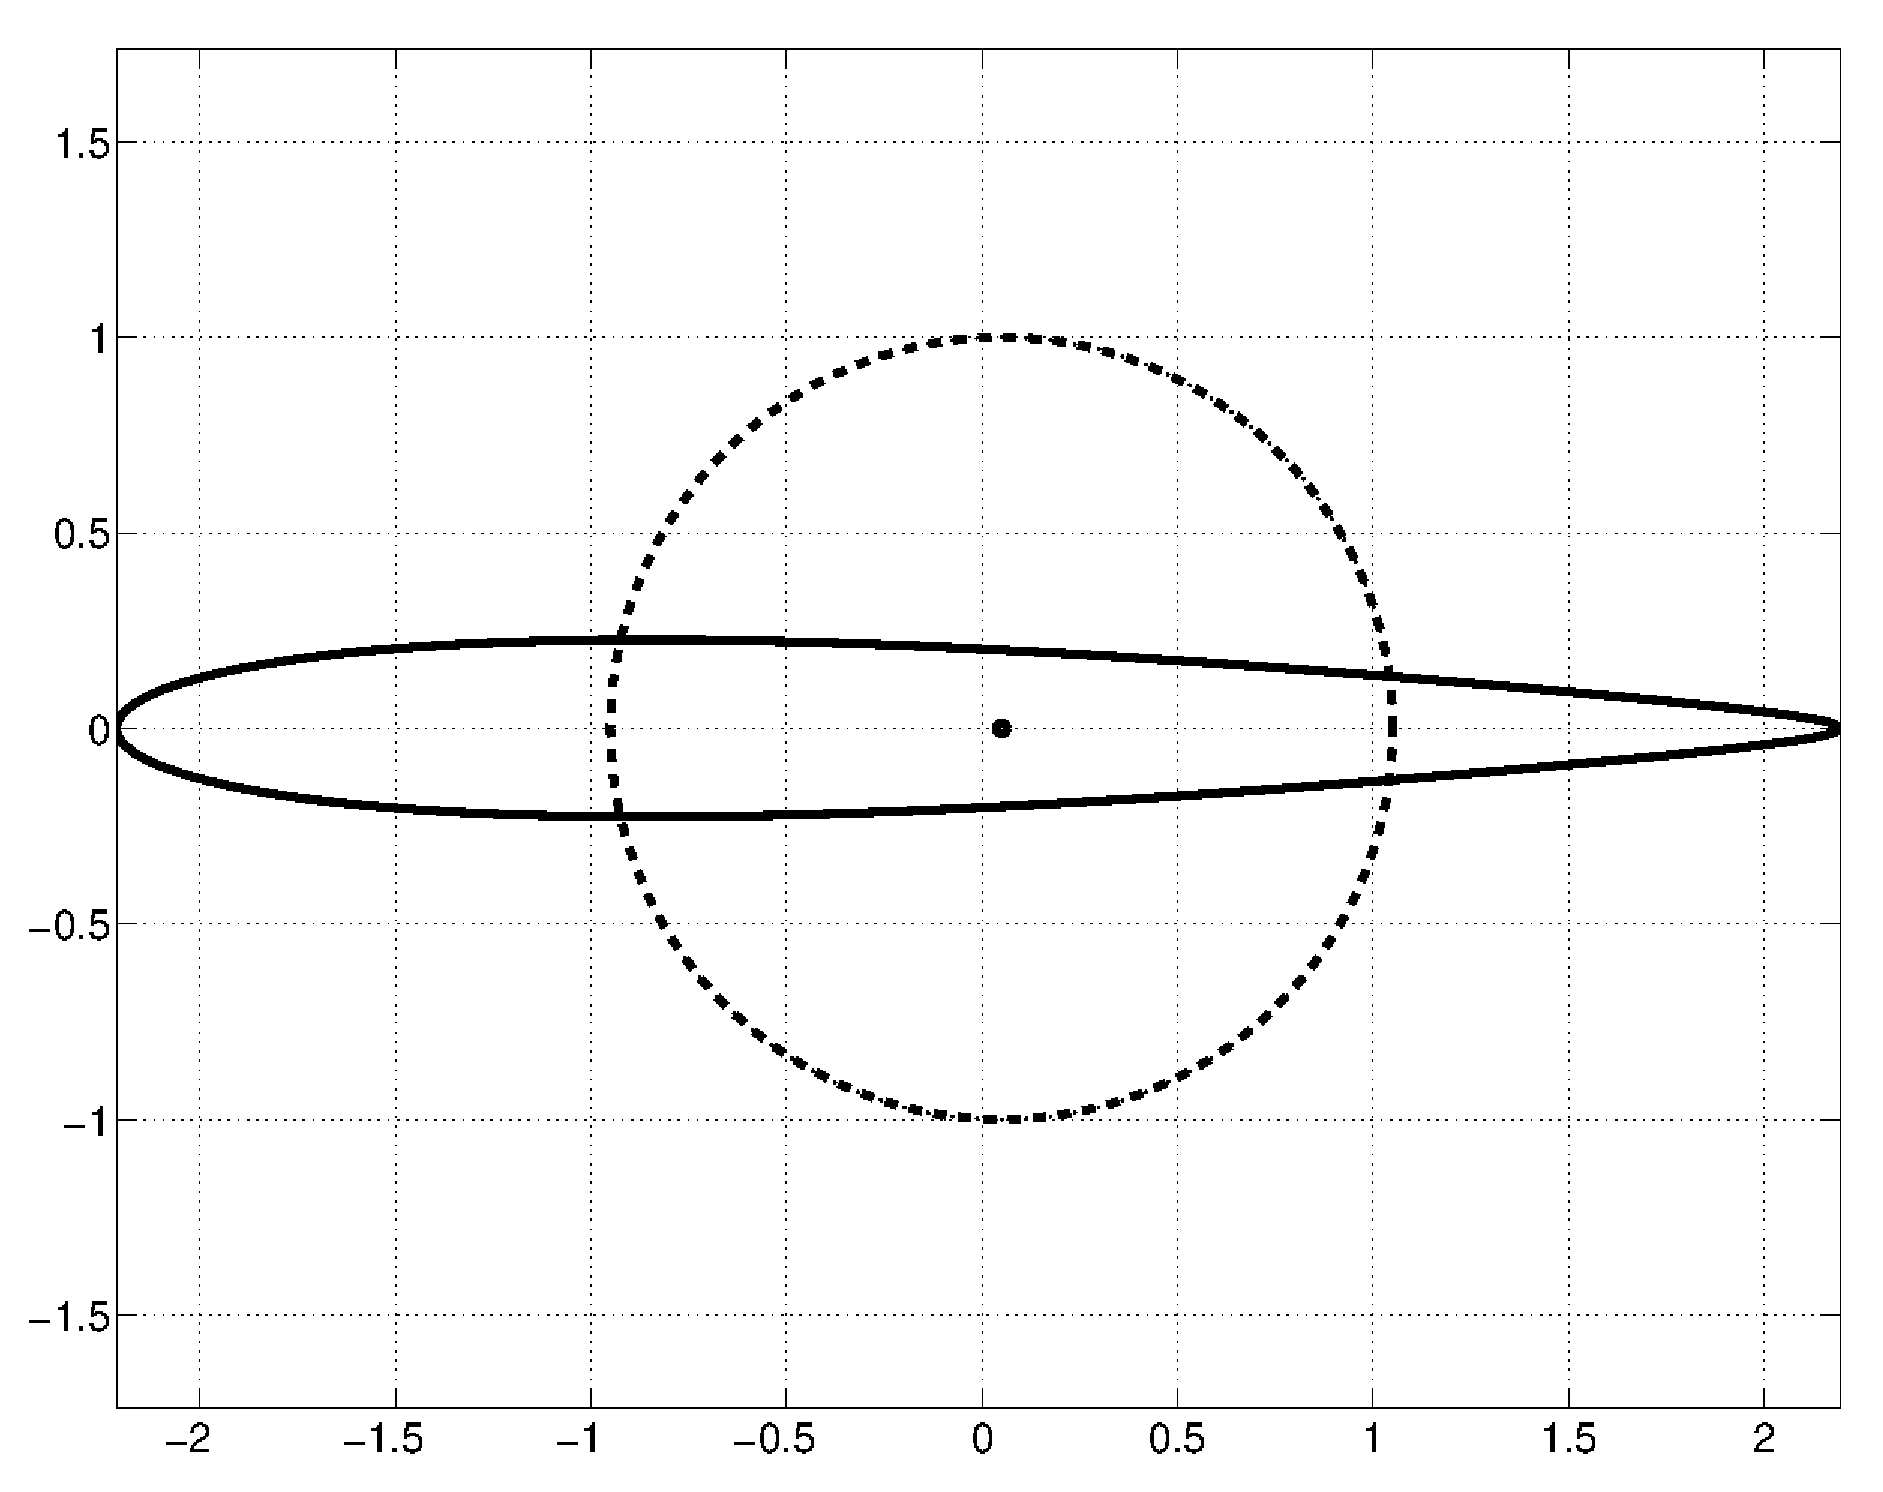
\includegraphics[width=4.25cm]{Chapter_5/figure/airfoil_base.eps}
    }
    \quad
    \subfigure[$x_c = 0.05, y_c = 0.1$]
    {
    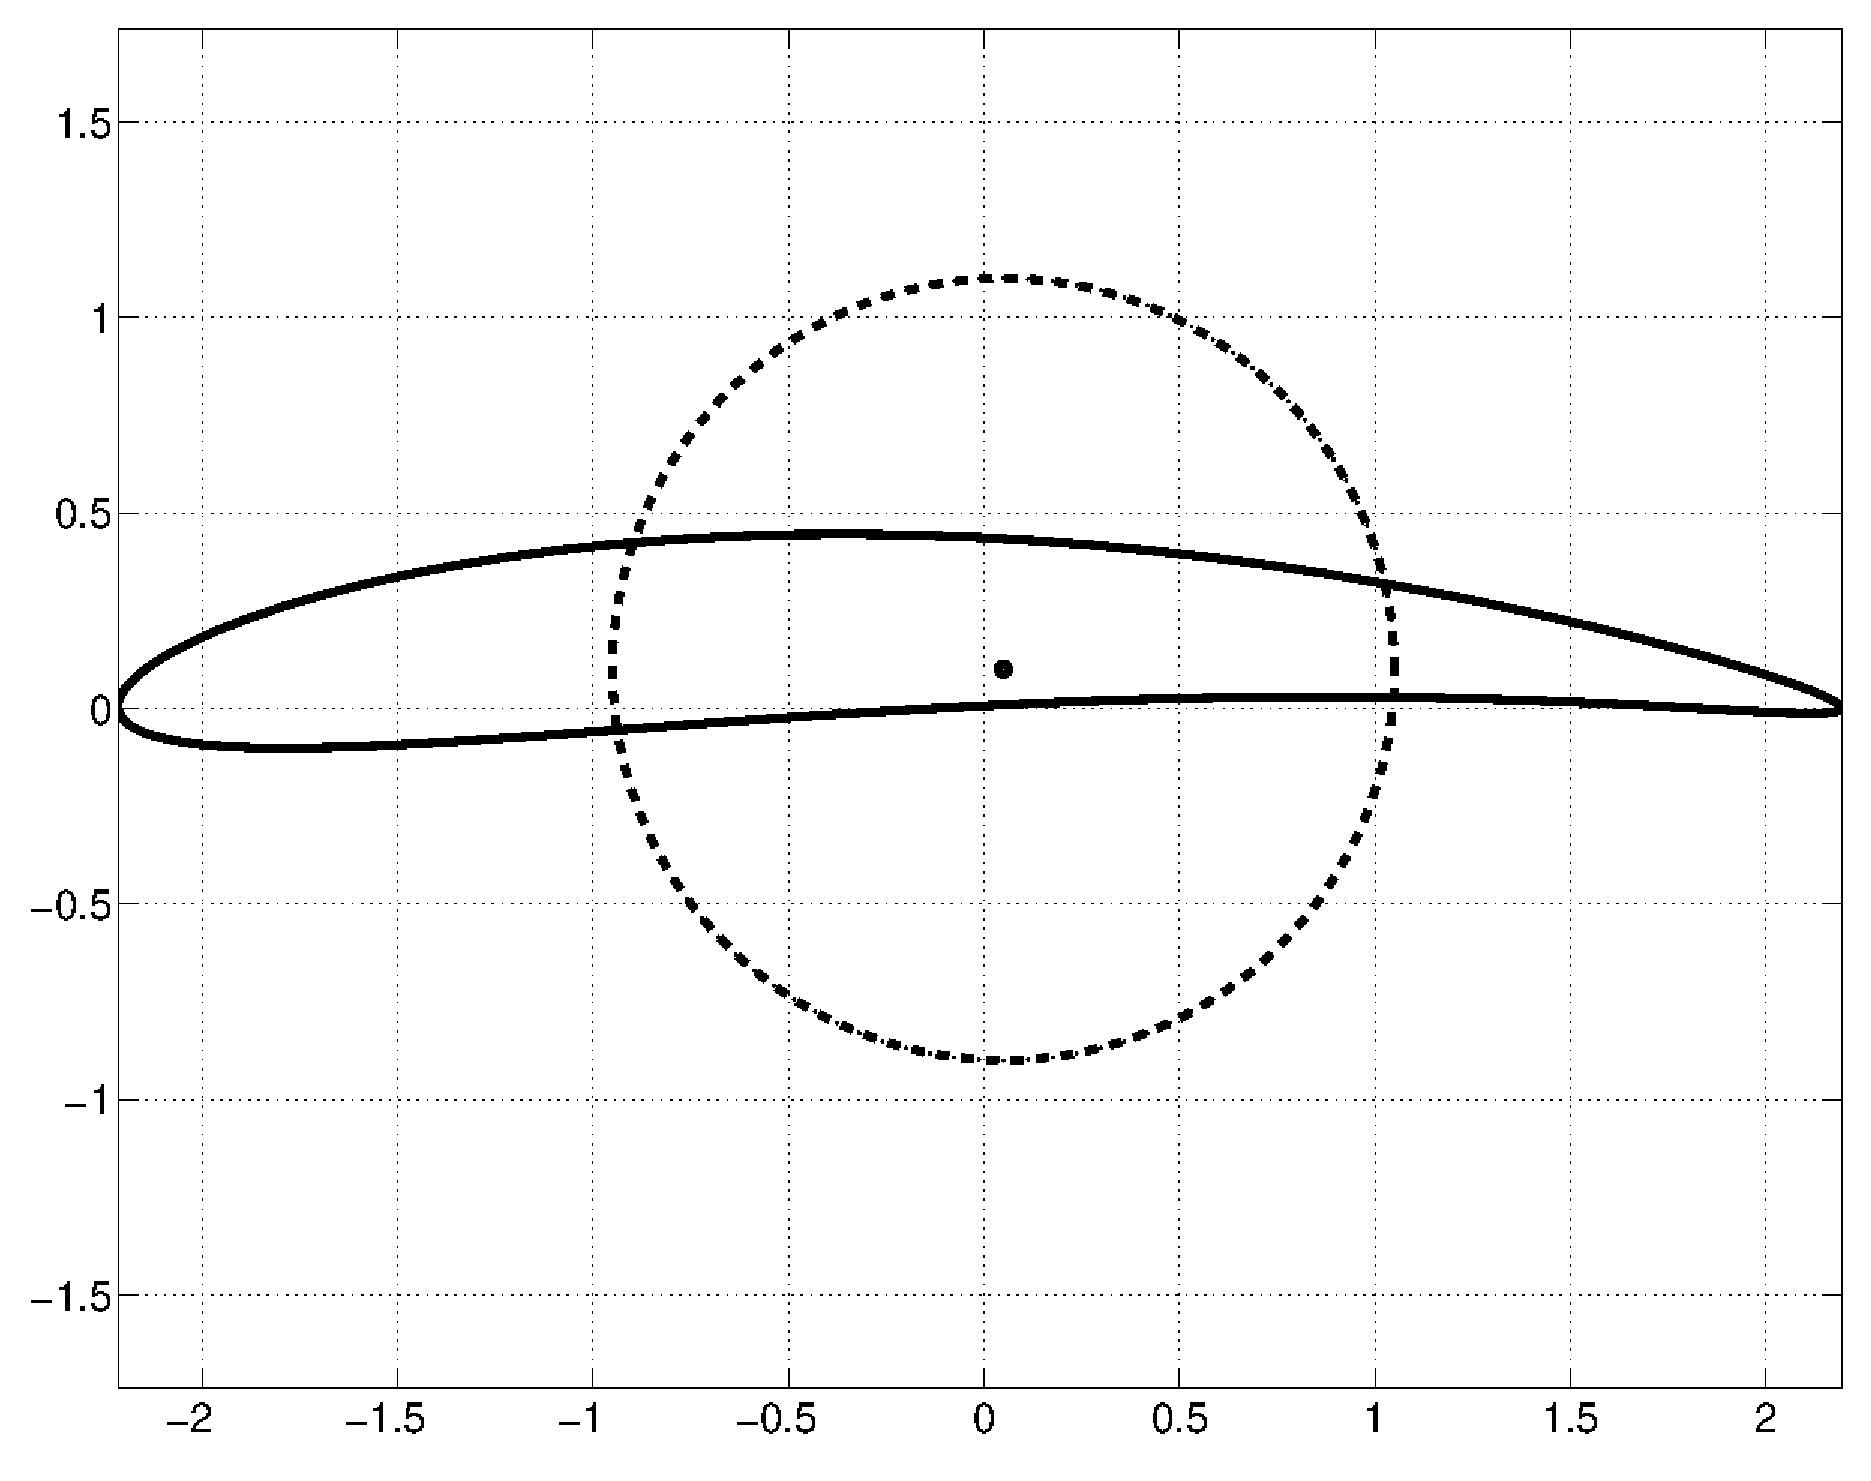
\includegraphics[width=4.25cm]{Chapter_5/figure/airfoil_camber.eps}
    }
    \quad
    \subfigure[$x_c = 0.1, y_c = 0.0$]
    {
    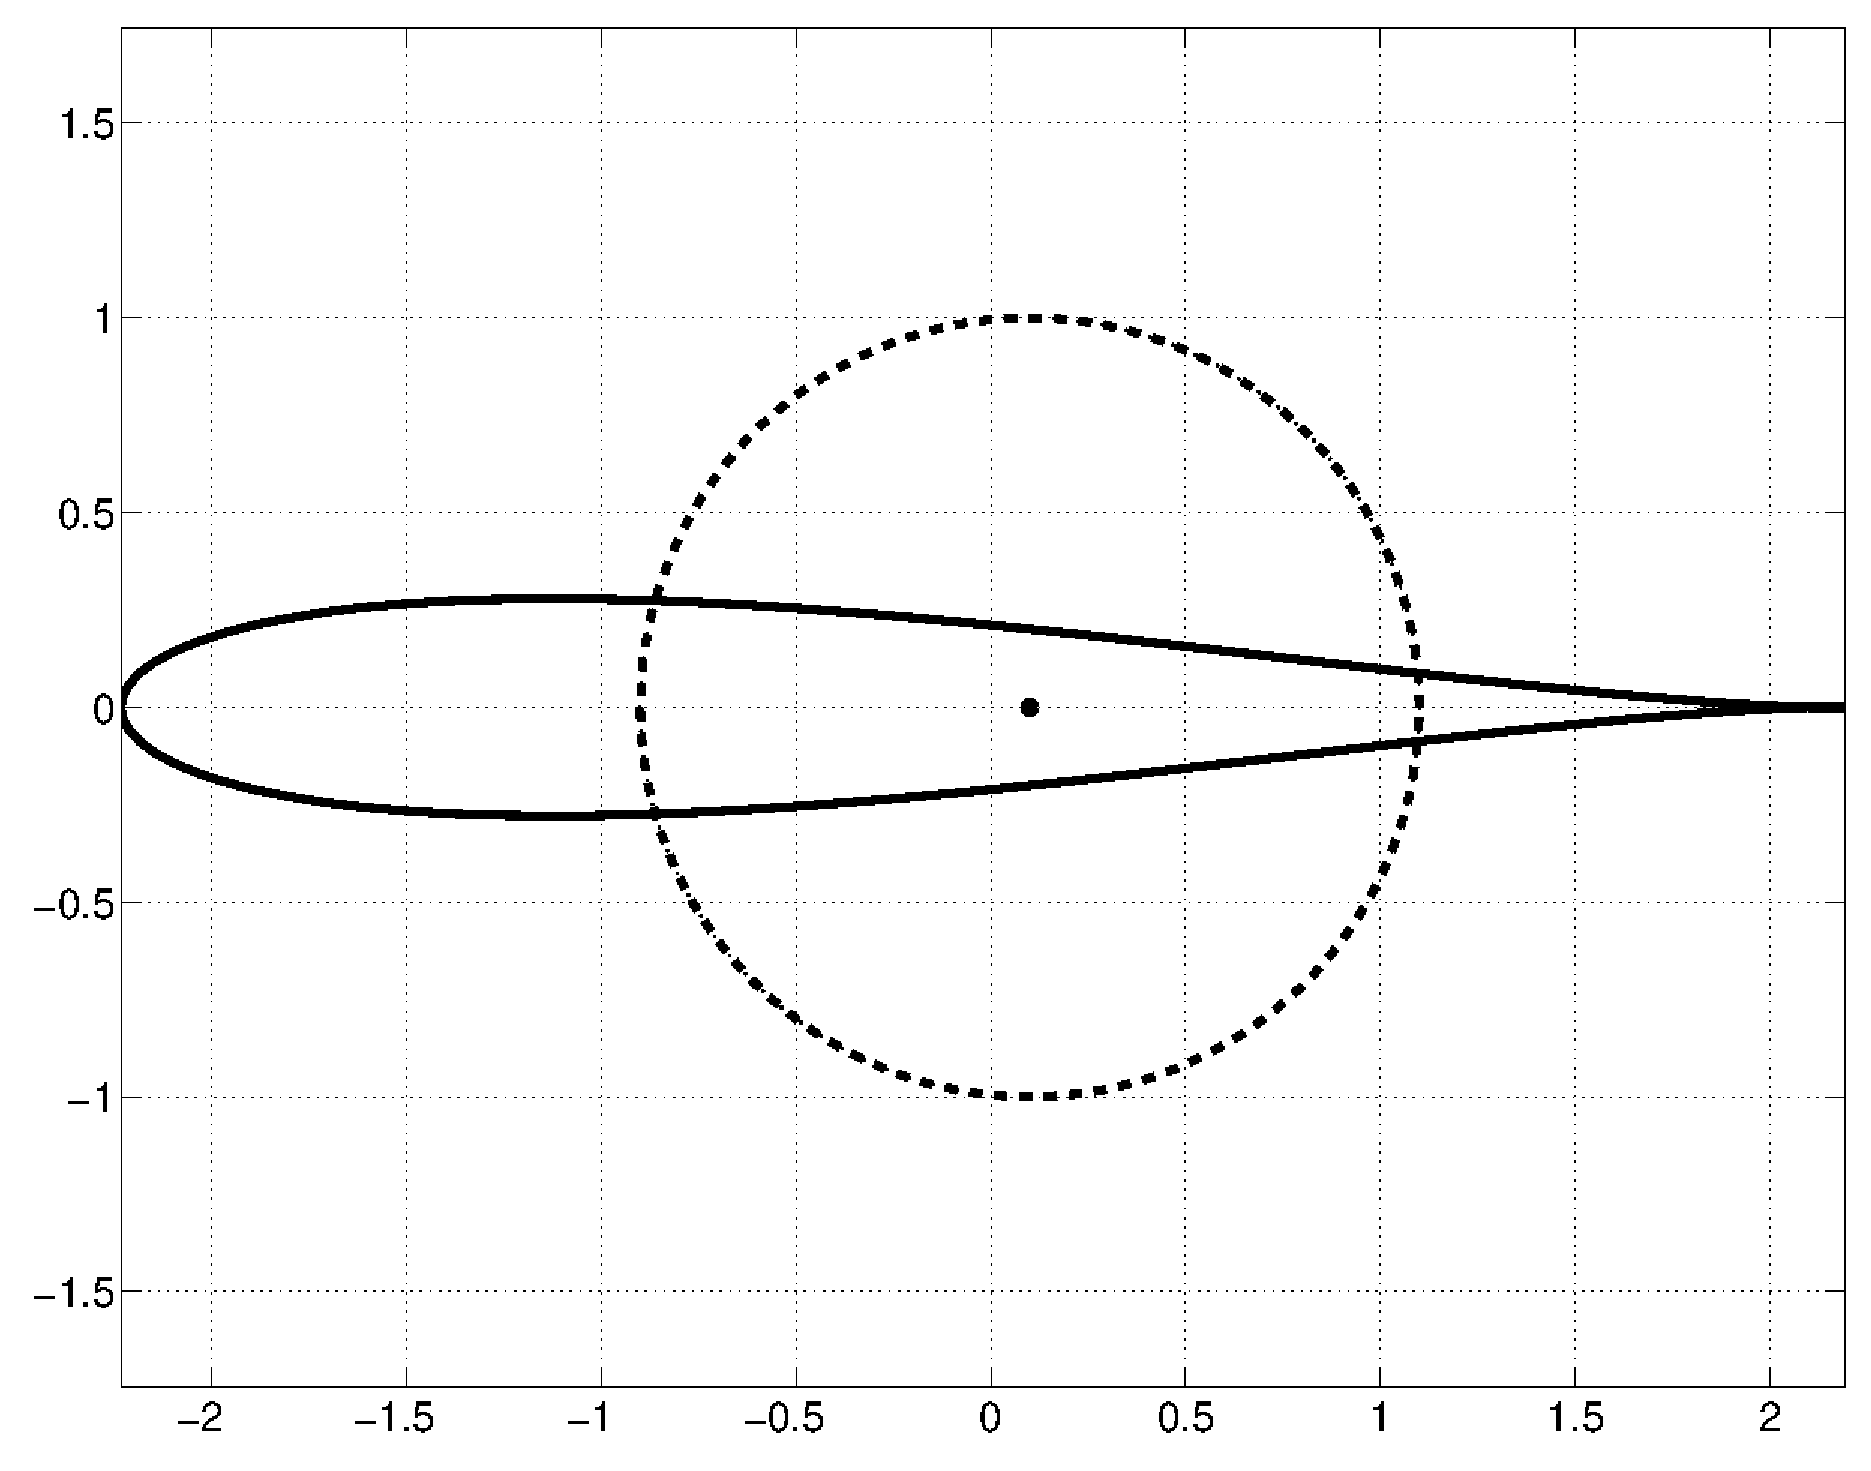
\includegraphics[width=4.25cm]{Chapter_5/figure/airfoil_thickness.eps}
    }
    \caption{Effect of circle location on Joukowsky airfoil shape.}
    \label{fig:C5_joukowskyAirfoil}
\end{figure}
%
The computational domain for this problem is defined as shown in Figure \ref{fig:C5_domainAirfoil}. The rigid airfoil is mounted on a two degree-of-freedom elastic structure as shown in Figure \ref{fig:C5_airfoilStructure}. The elastic structure contains a axial and torsional spring to better represent and actual wing.
%
\begin{figure}[H]
    \centering
    \subfigure[Physical domain.]
    {
    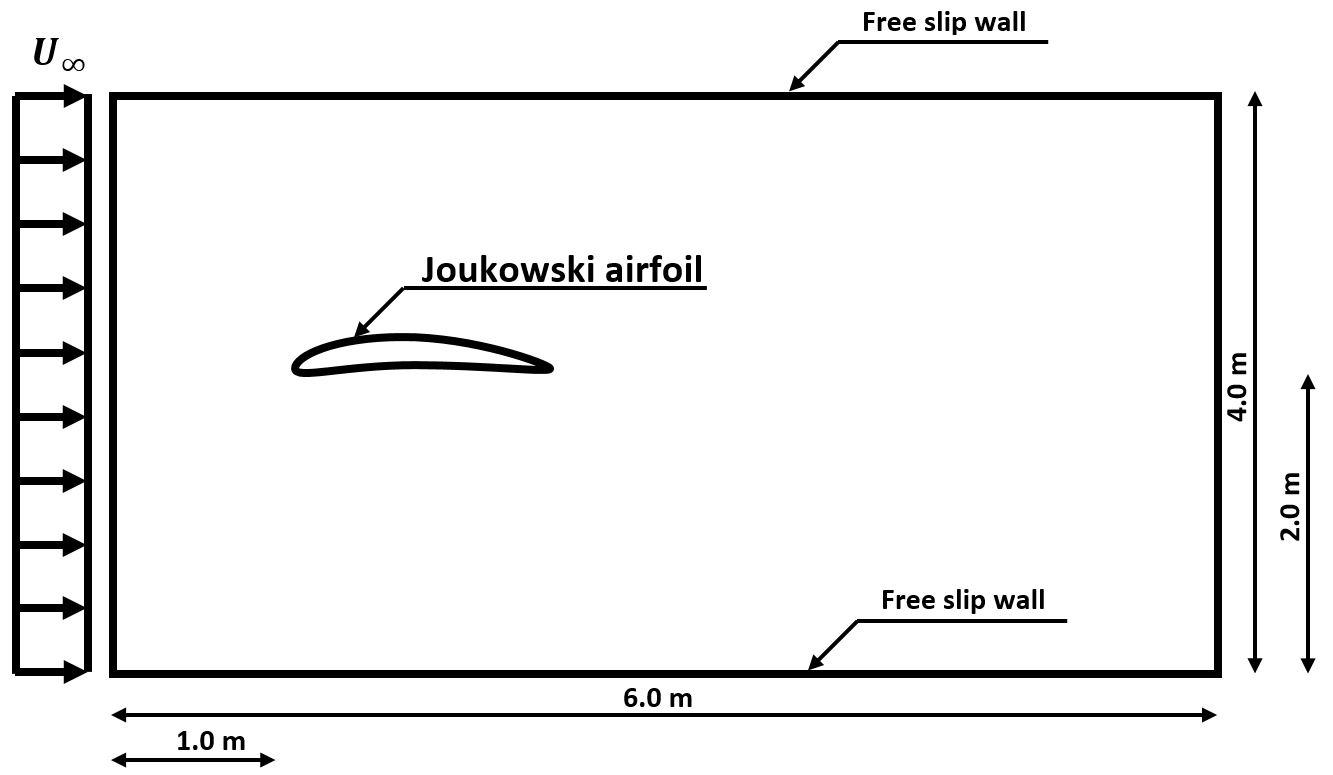
\includegraphics[width=8cm]{Chapter_5/figure/airfoilPhysicalDomain.JPG}
    \label{fig:C5_domainAirfoil}
    }
    \quad
    \subfigure[Airfoil elastic structure]
    {
    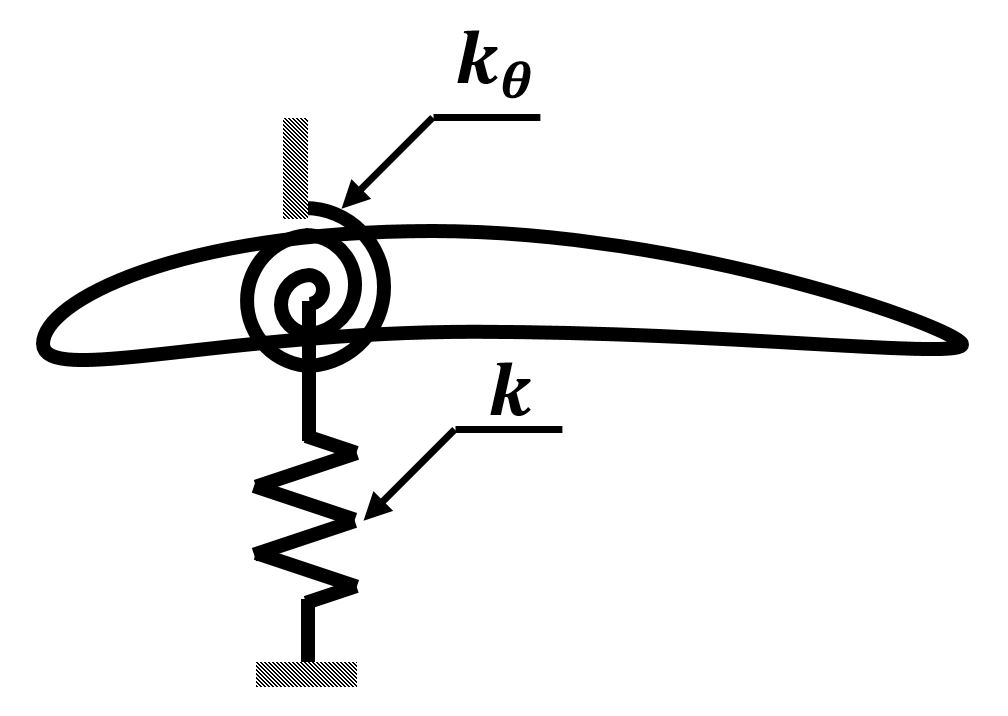
\includegraphics[width=5cm]{Chapter_5/figure/airfoilStructure.JPG}
    \label{fig:C5_airfoilStructure}
    }
    \caption{Physical domain and elastic structure for the pitching and plunging airfoil.}
\end{figure}
%
For this problem we look at two different airfoils mounted on the elastic structure as shown in Figure \ref{fig:C5_airfoilShape}. The difference in airfoil shape will result in different characteristics in the FSI response of the system. From now we refer to the airfoil defined in Figure \ref{fig:C5_thinAirfoil} as \emph{thin airfoil} and the one in Figure \ref{fig:C5_thickAirfoil} as \emph{thick airfoil}.
%
\begin{figure}[H]
    \centering
    \subfigure[$x_c = 0.05, y_c = 0.1$]
    {
    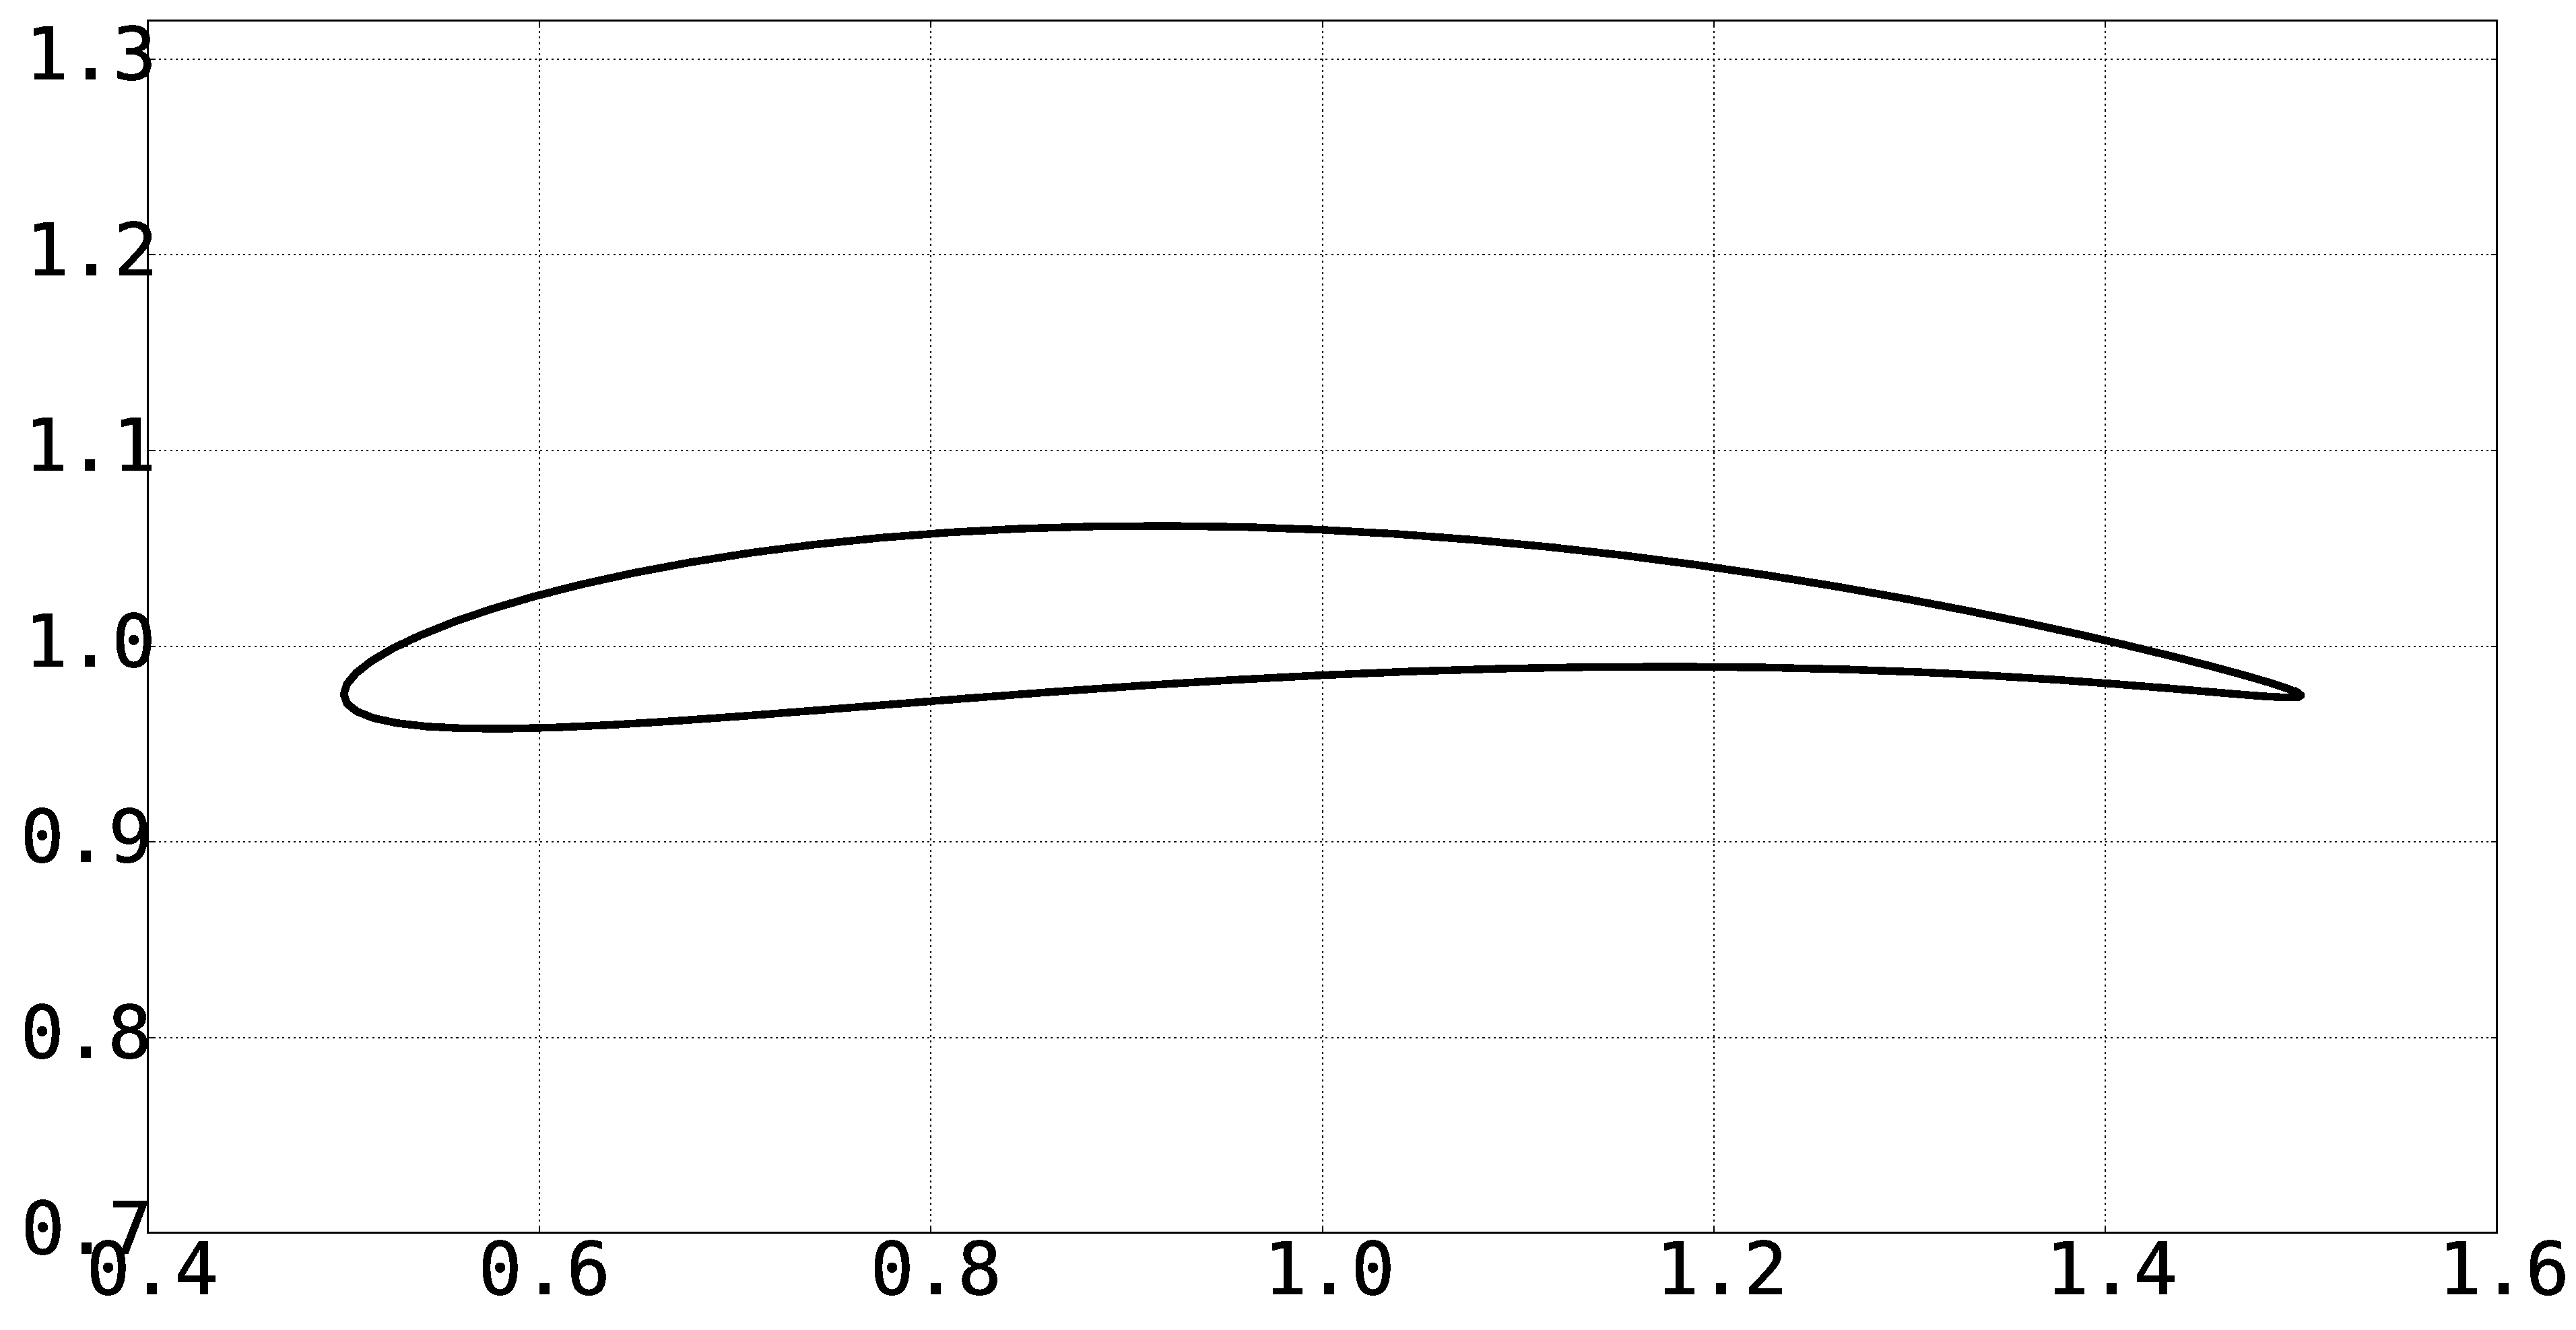
\includegraphics[width=6.5cm]{Chapter_5/figure/airfoil1.eps}
    \label{fig:C5_thinAirfoil}
    }
    \quad
    \subfigure[$x_c = 0.1, y_c = 0.2$]
    {
    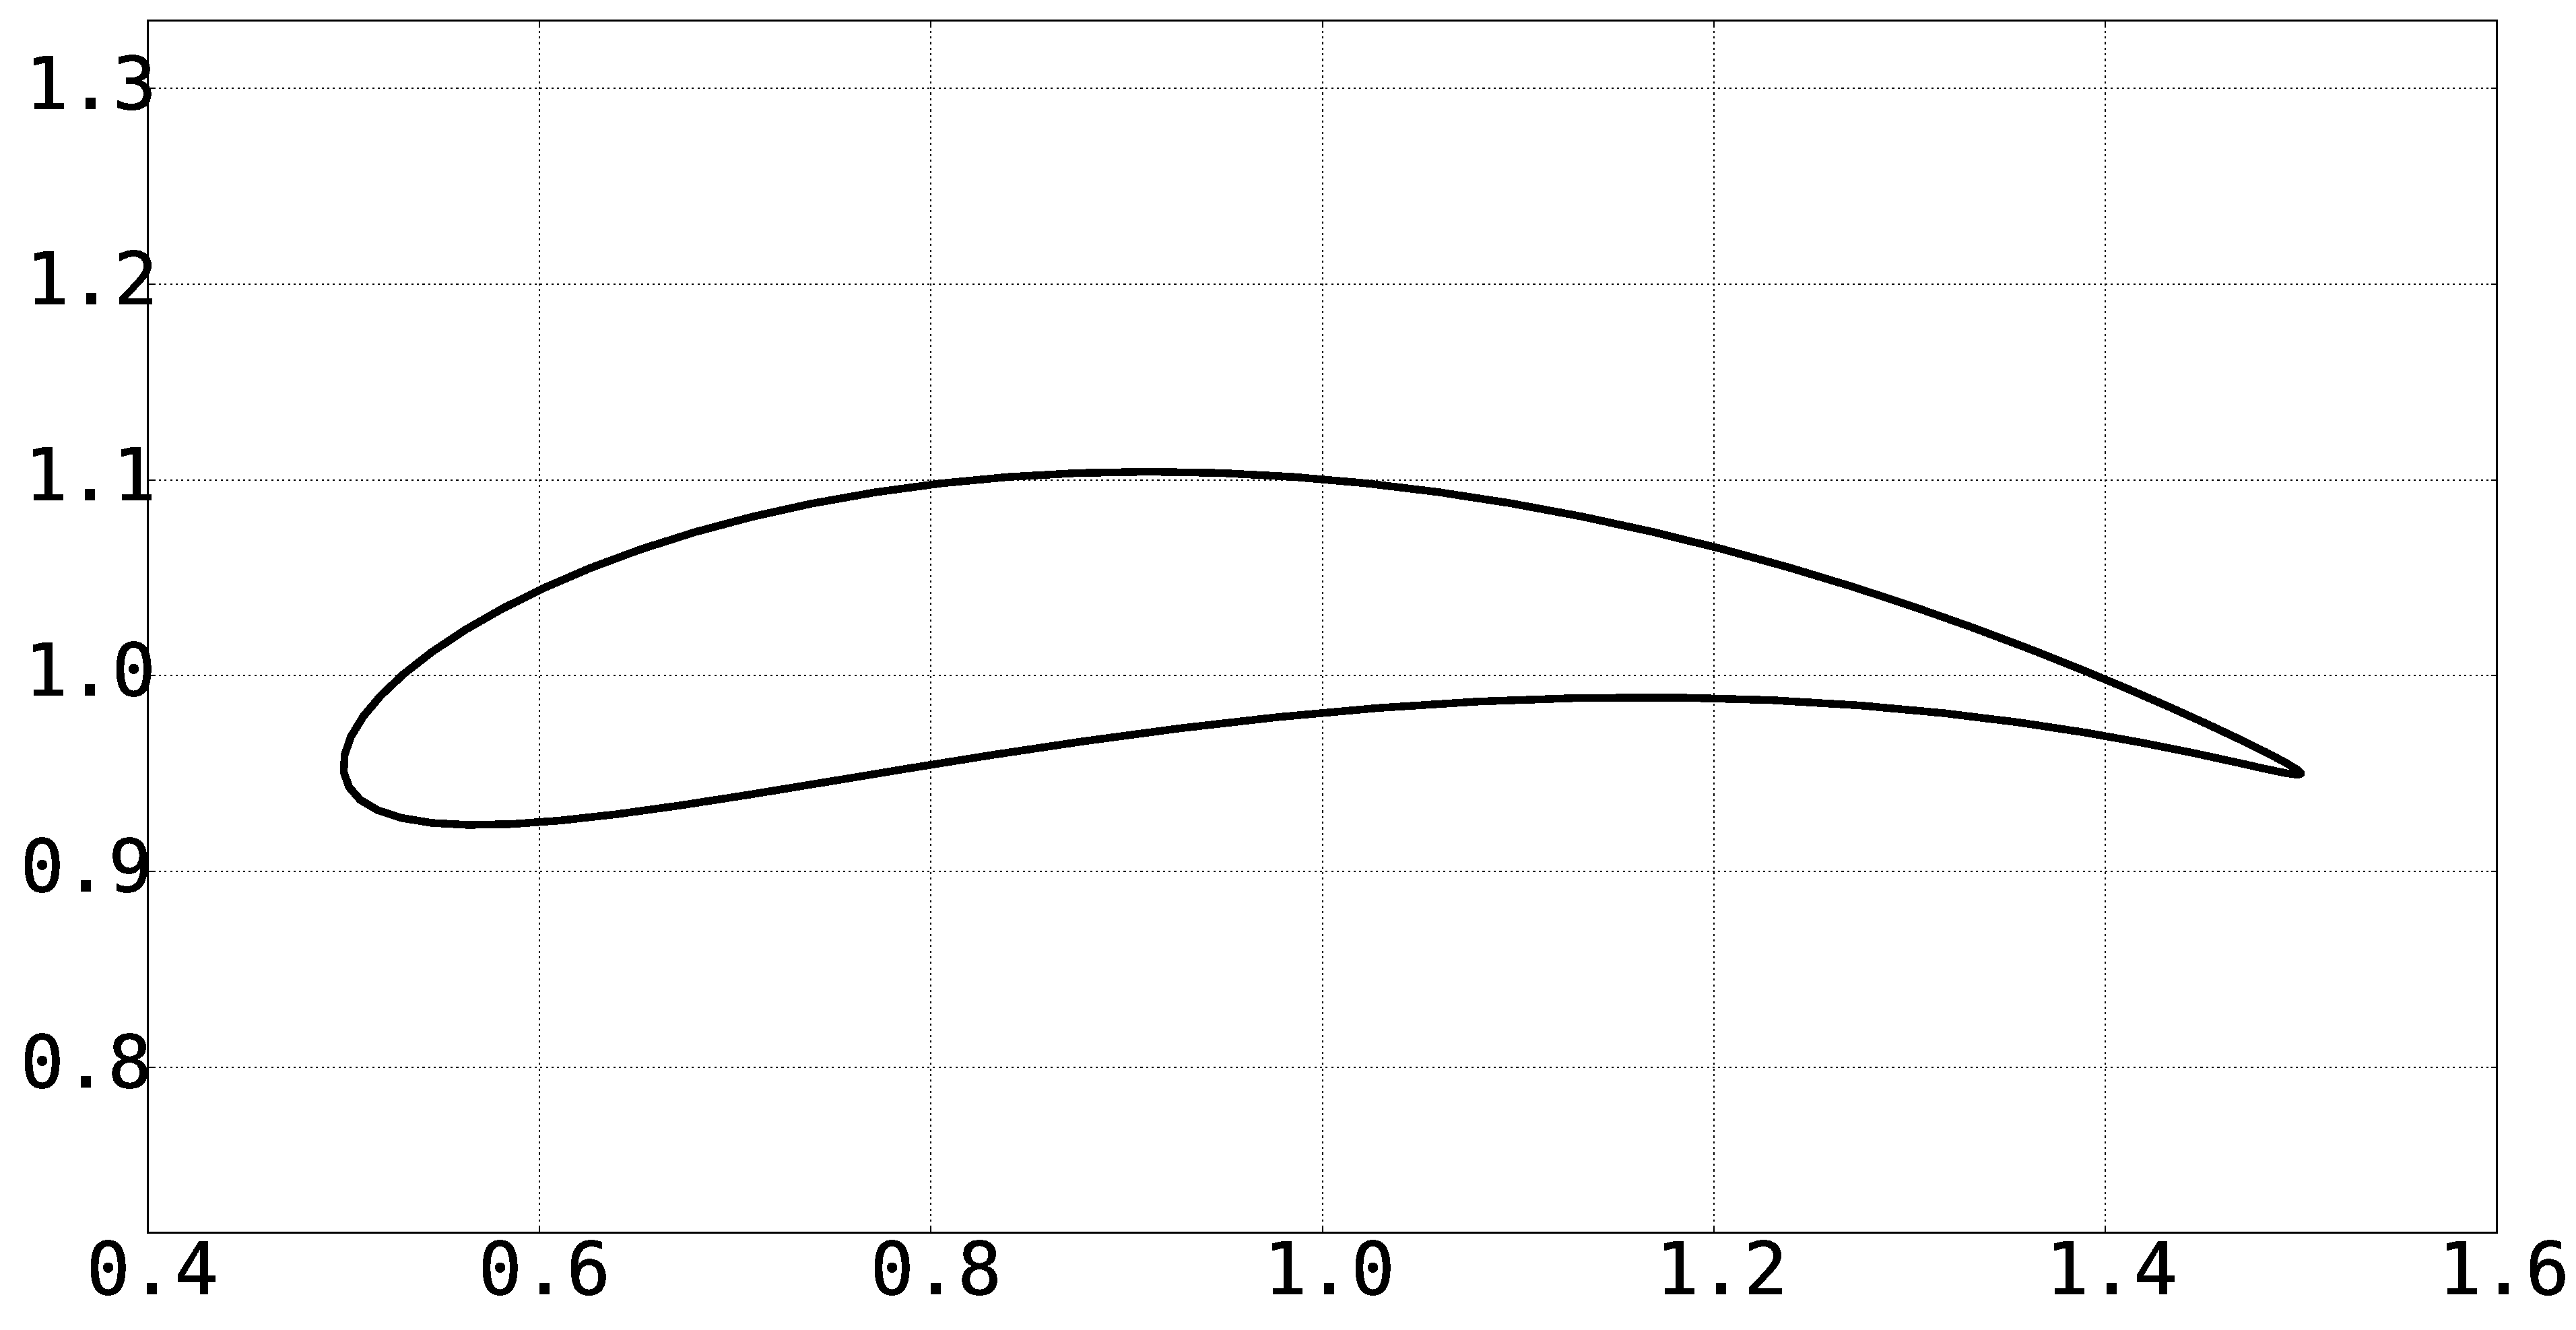
\includegraphics[width=6.5cm]{Chapter_5/figure/airfoil2.eps}
    \label{fig:C5_thickAirfoil}
    }
    \caption{Airfoil shape used for FSI calculation.}
    \label{fig:C5_airfoilShape}
\end{figure}
%
The Reynolds number for this simulation is selected as $100$. Higher Reynolds number will result in turbulent flow which is not considered in this research and therefore the solution results for higher Reynolds numbers does not represent a physical solution. For the elastic structure properties, spring stiffness is selected as $0.5 N/m$, airfoil mass as $1.0 Kg$, rotational spring as $0.1 N/\theta$, and the moment of inertia as $1.0 Kg \cdot m^2$. The results for the first 50 second simulation of the airfoil center location and change in the angle of attack due to aerodynamic loads are shown in Figure \ref{fig:C5_airfoilDisplacementRotation}. As shown here, the thin airfoil of Figure \ref{fig:C5_thinAirfoil} follows an oscillatory response whereas the thick airfoil of Figure \ref{fig:C5_thickAirfoil} experience divergence.
%
\begin{figure}[H]
    \centering
    \subfigure[Thin airfoil displacement]
    {
    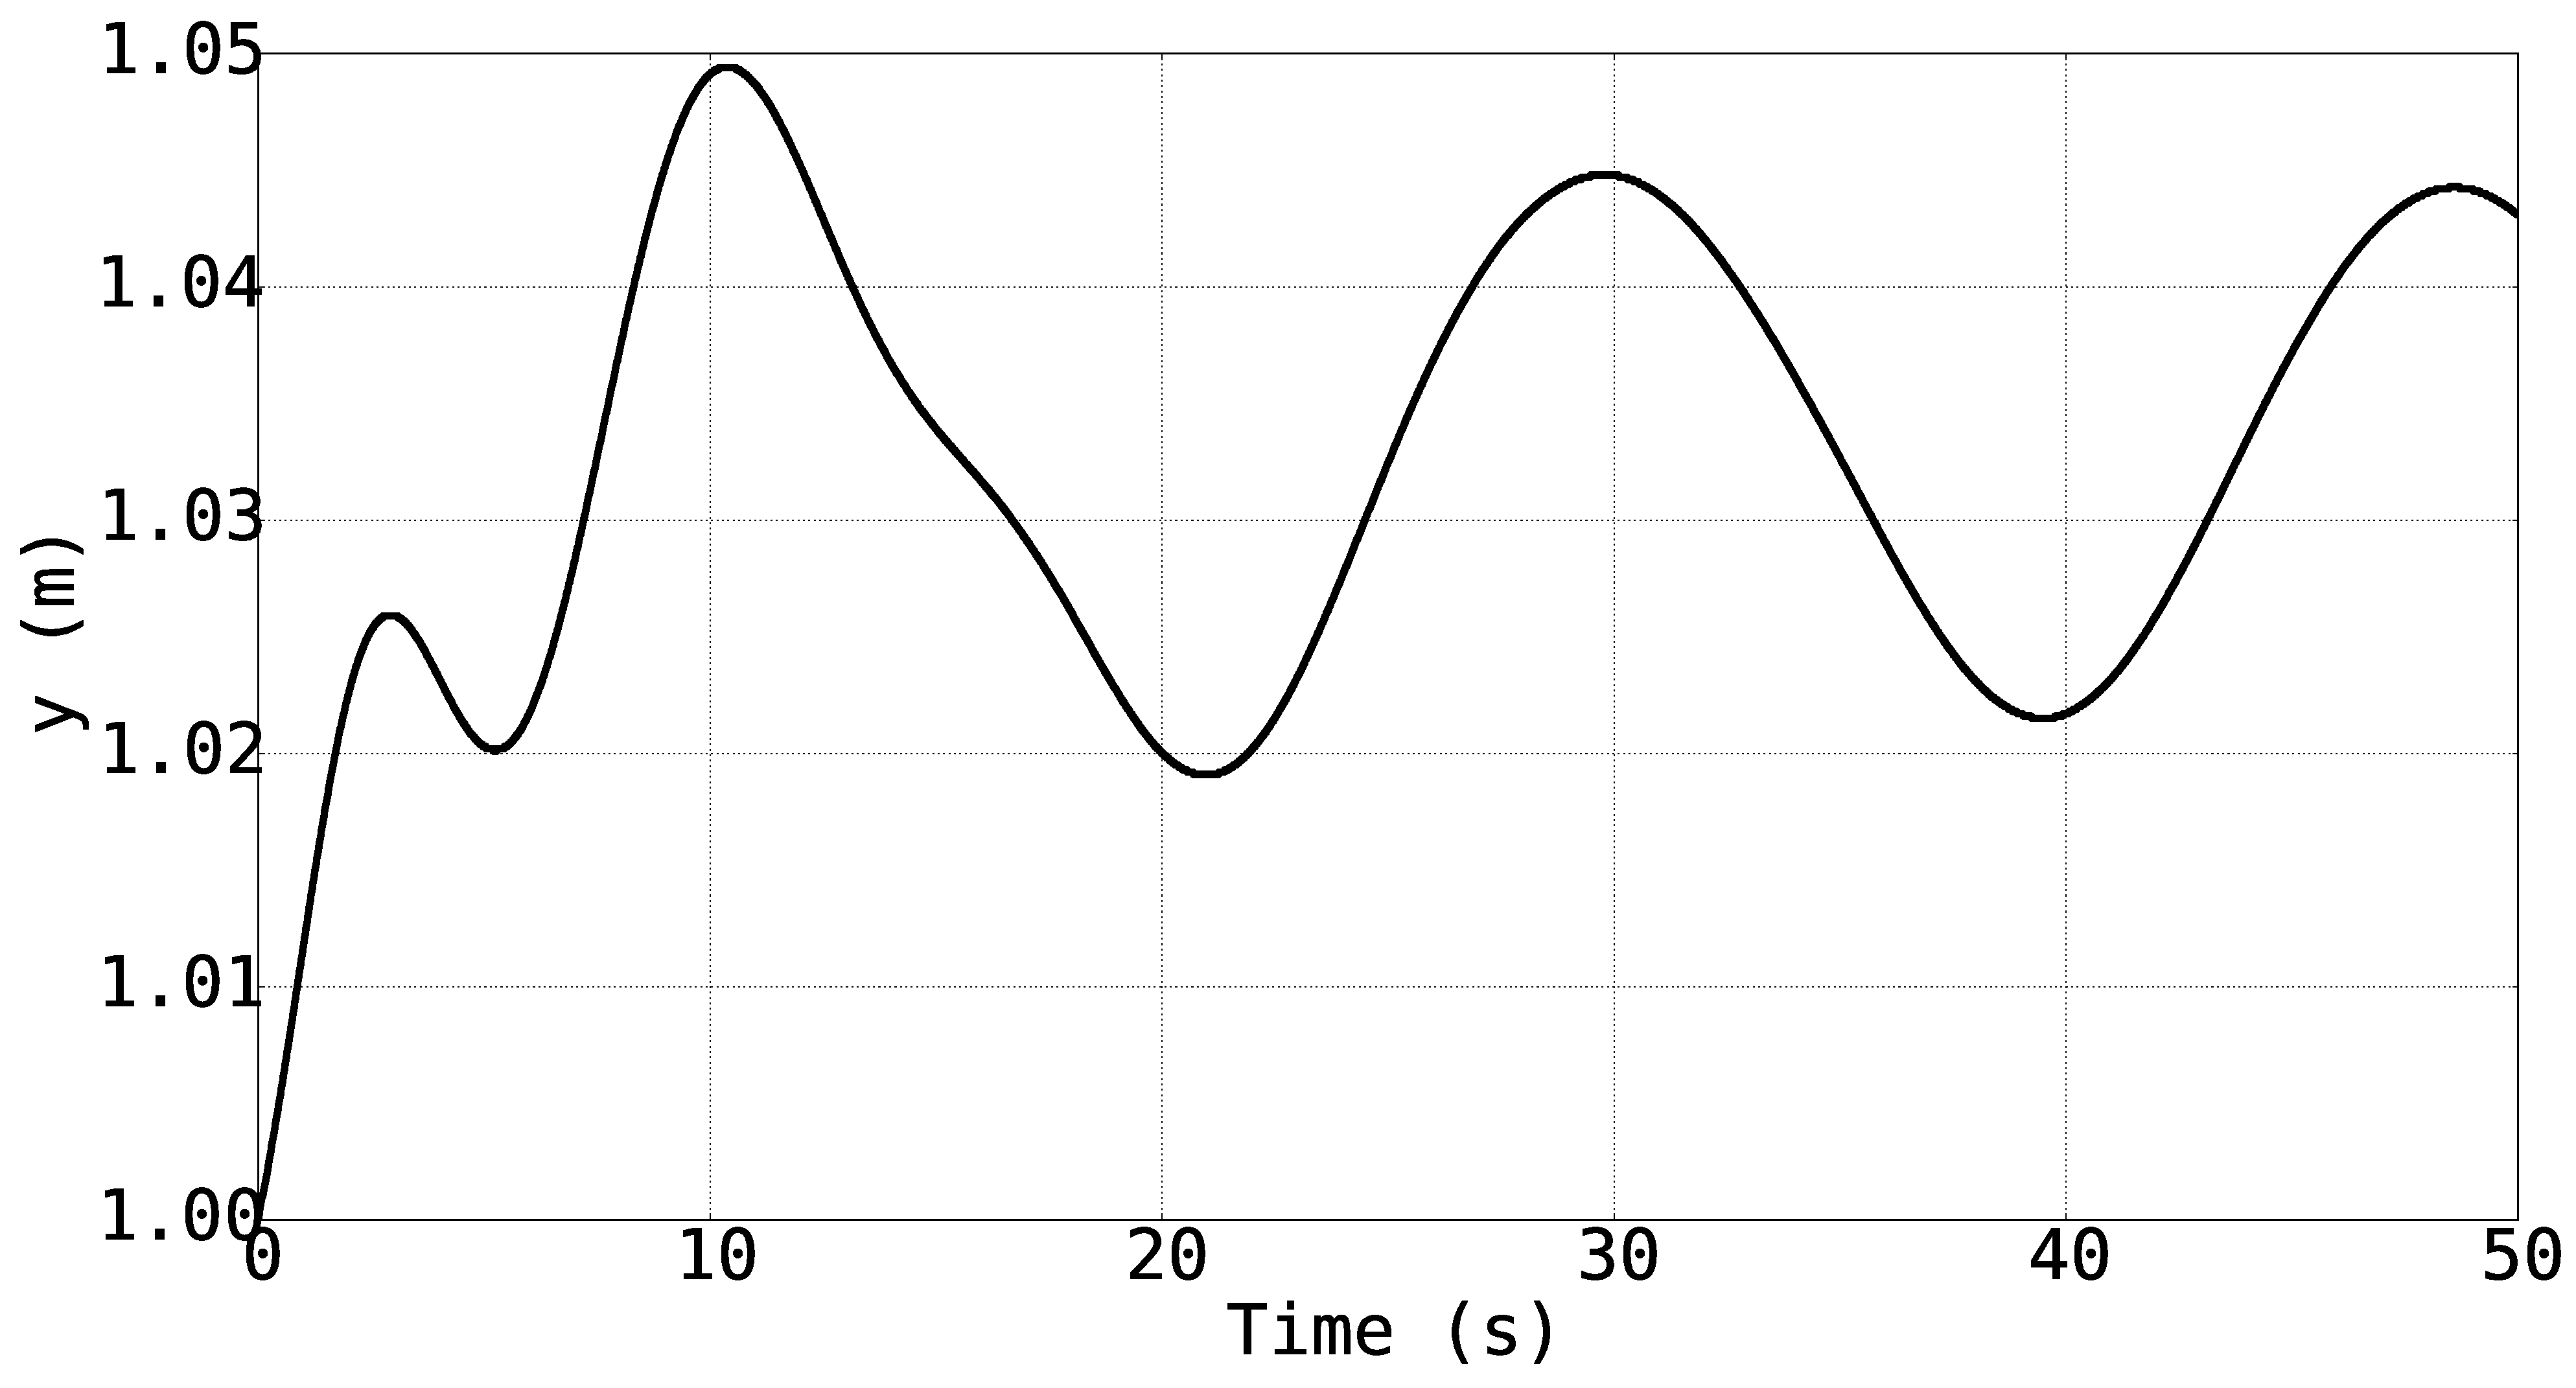
\includegraphics[width=6.5cm]{Chapter_5/figure/airfoil1_displacement.eps}
    }
    \quad
    \subfigure[Thick airfoil displacement]
    {
    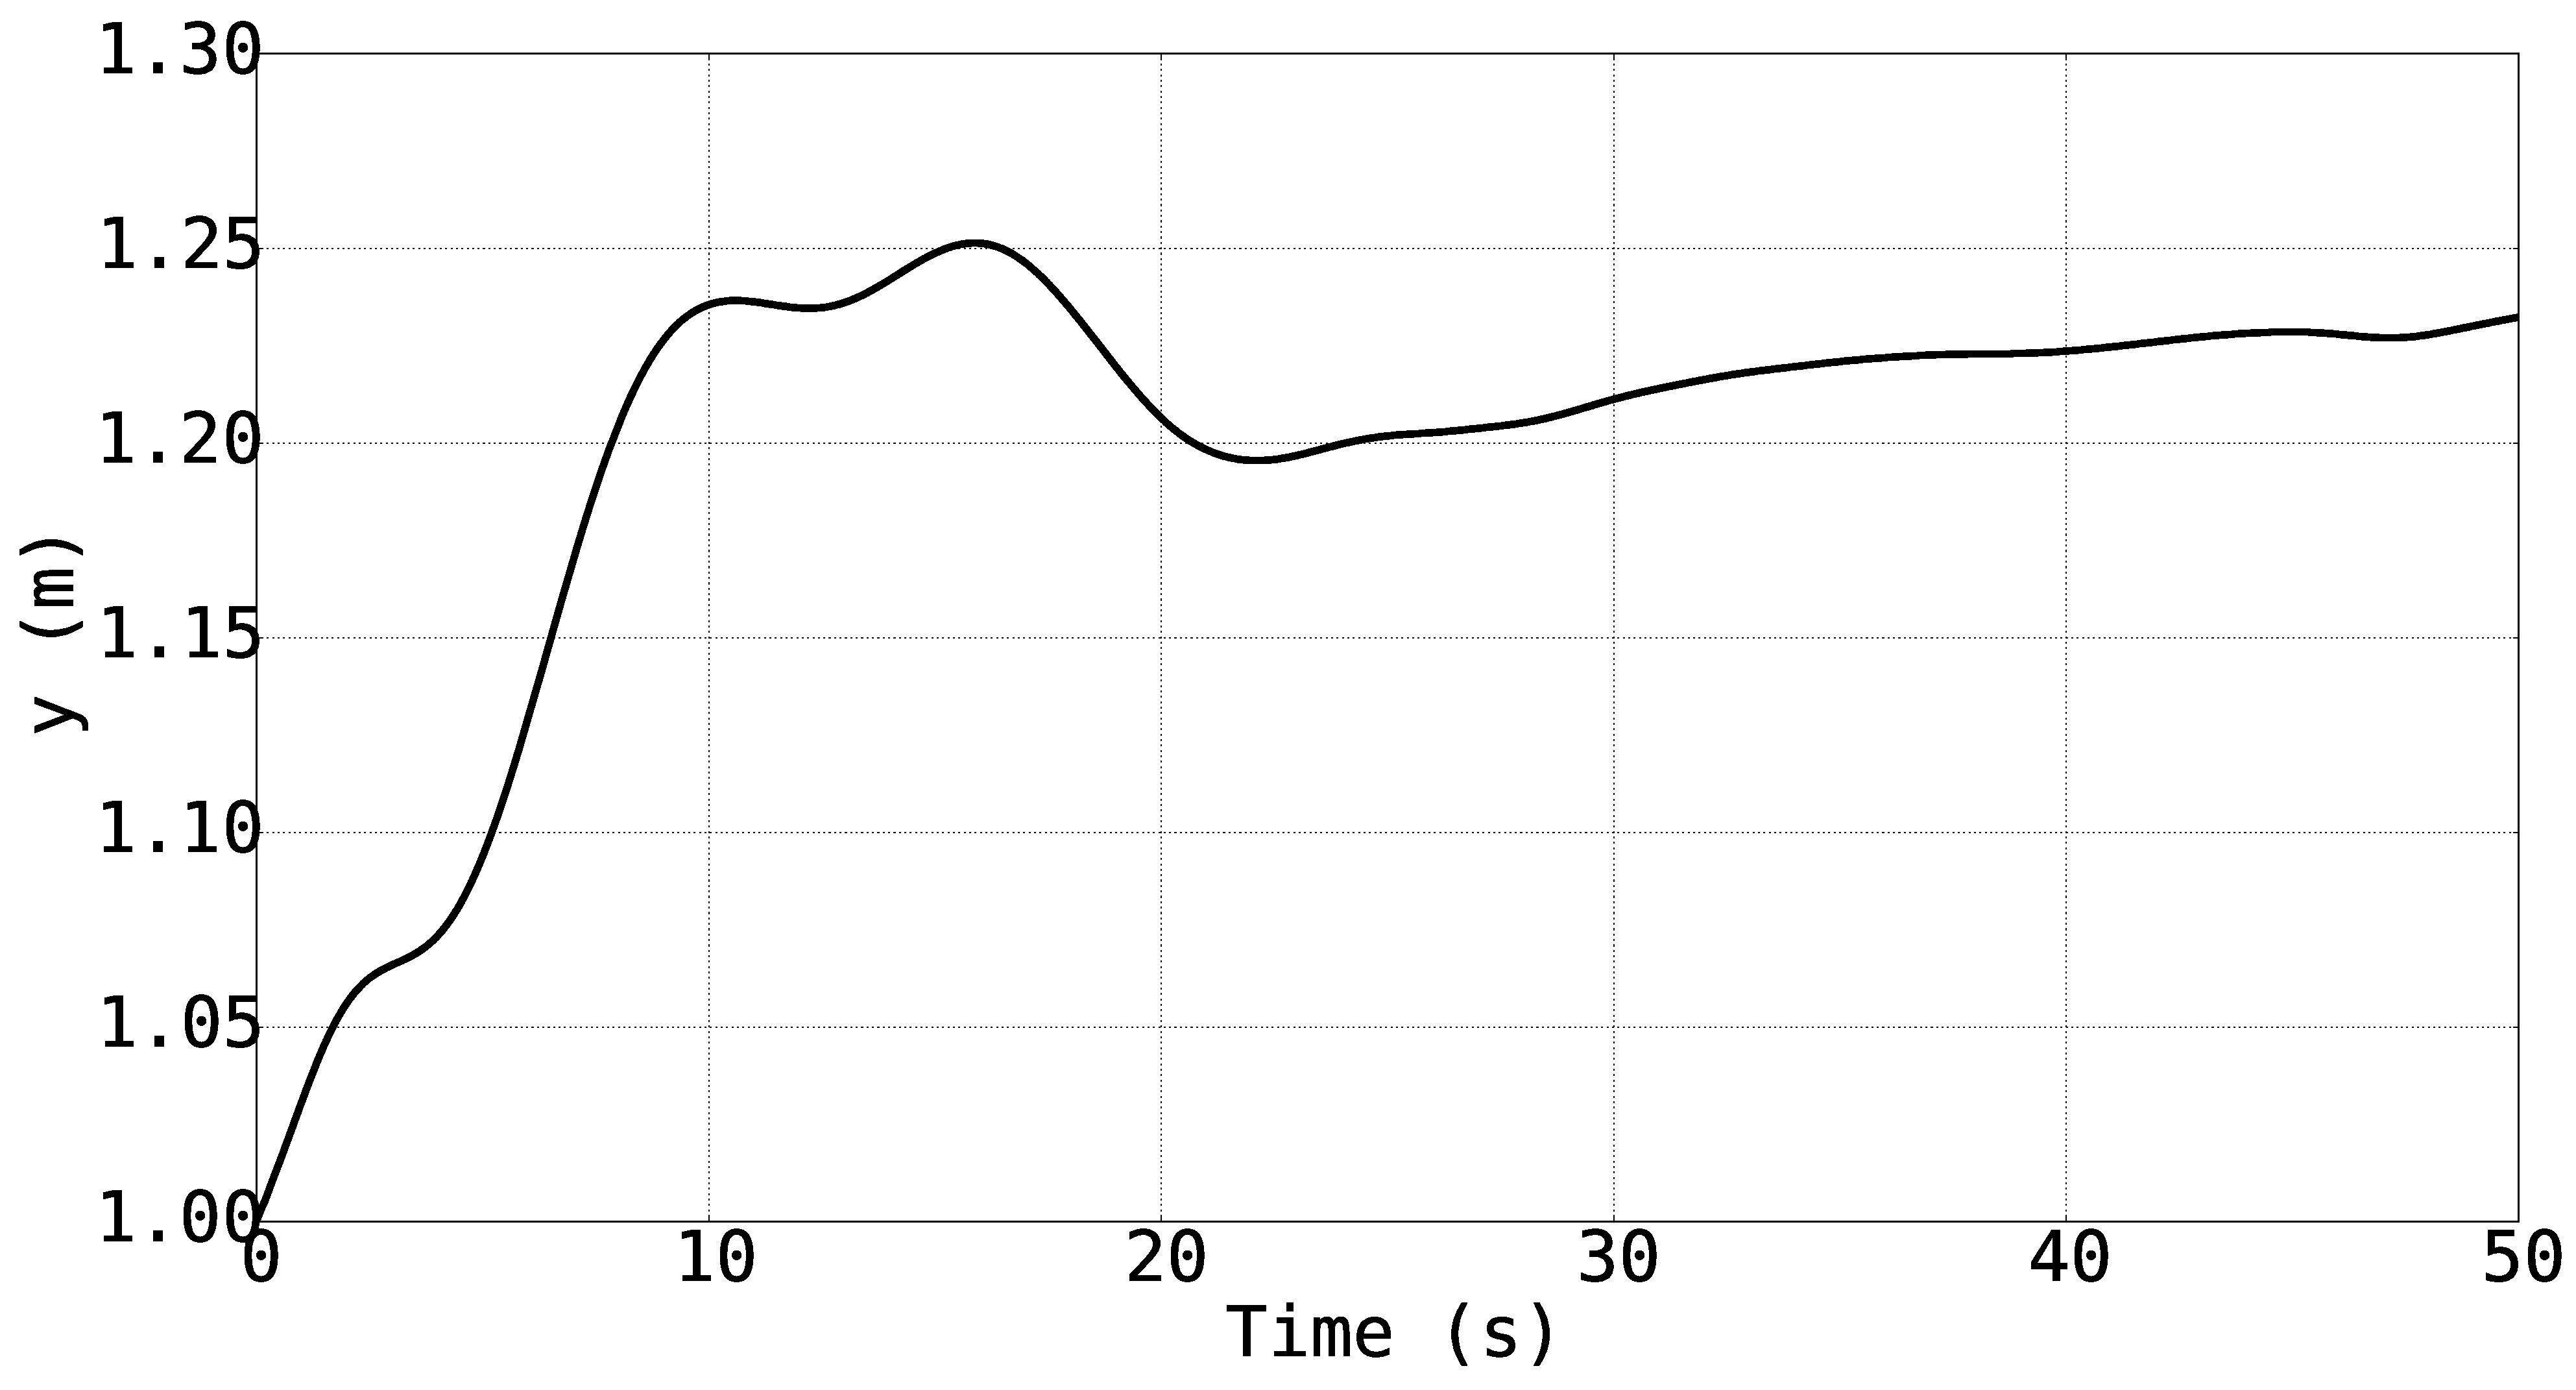
\includegraphics[width=6.5cm]{Chapter_5/figure/airfoil2_displacement.eps}
    }
    \\
    \subfigure[Thin airfoil rotation]
    {
    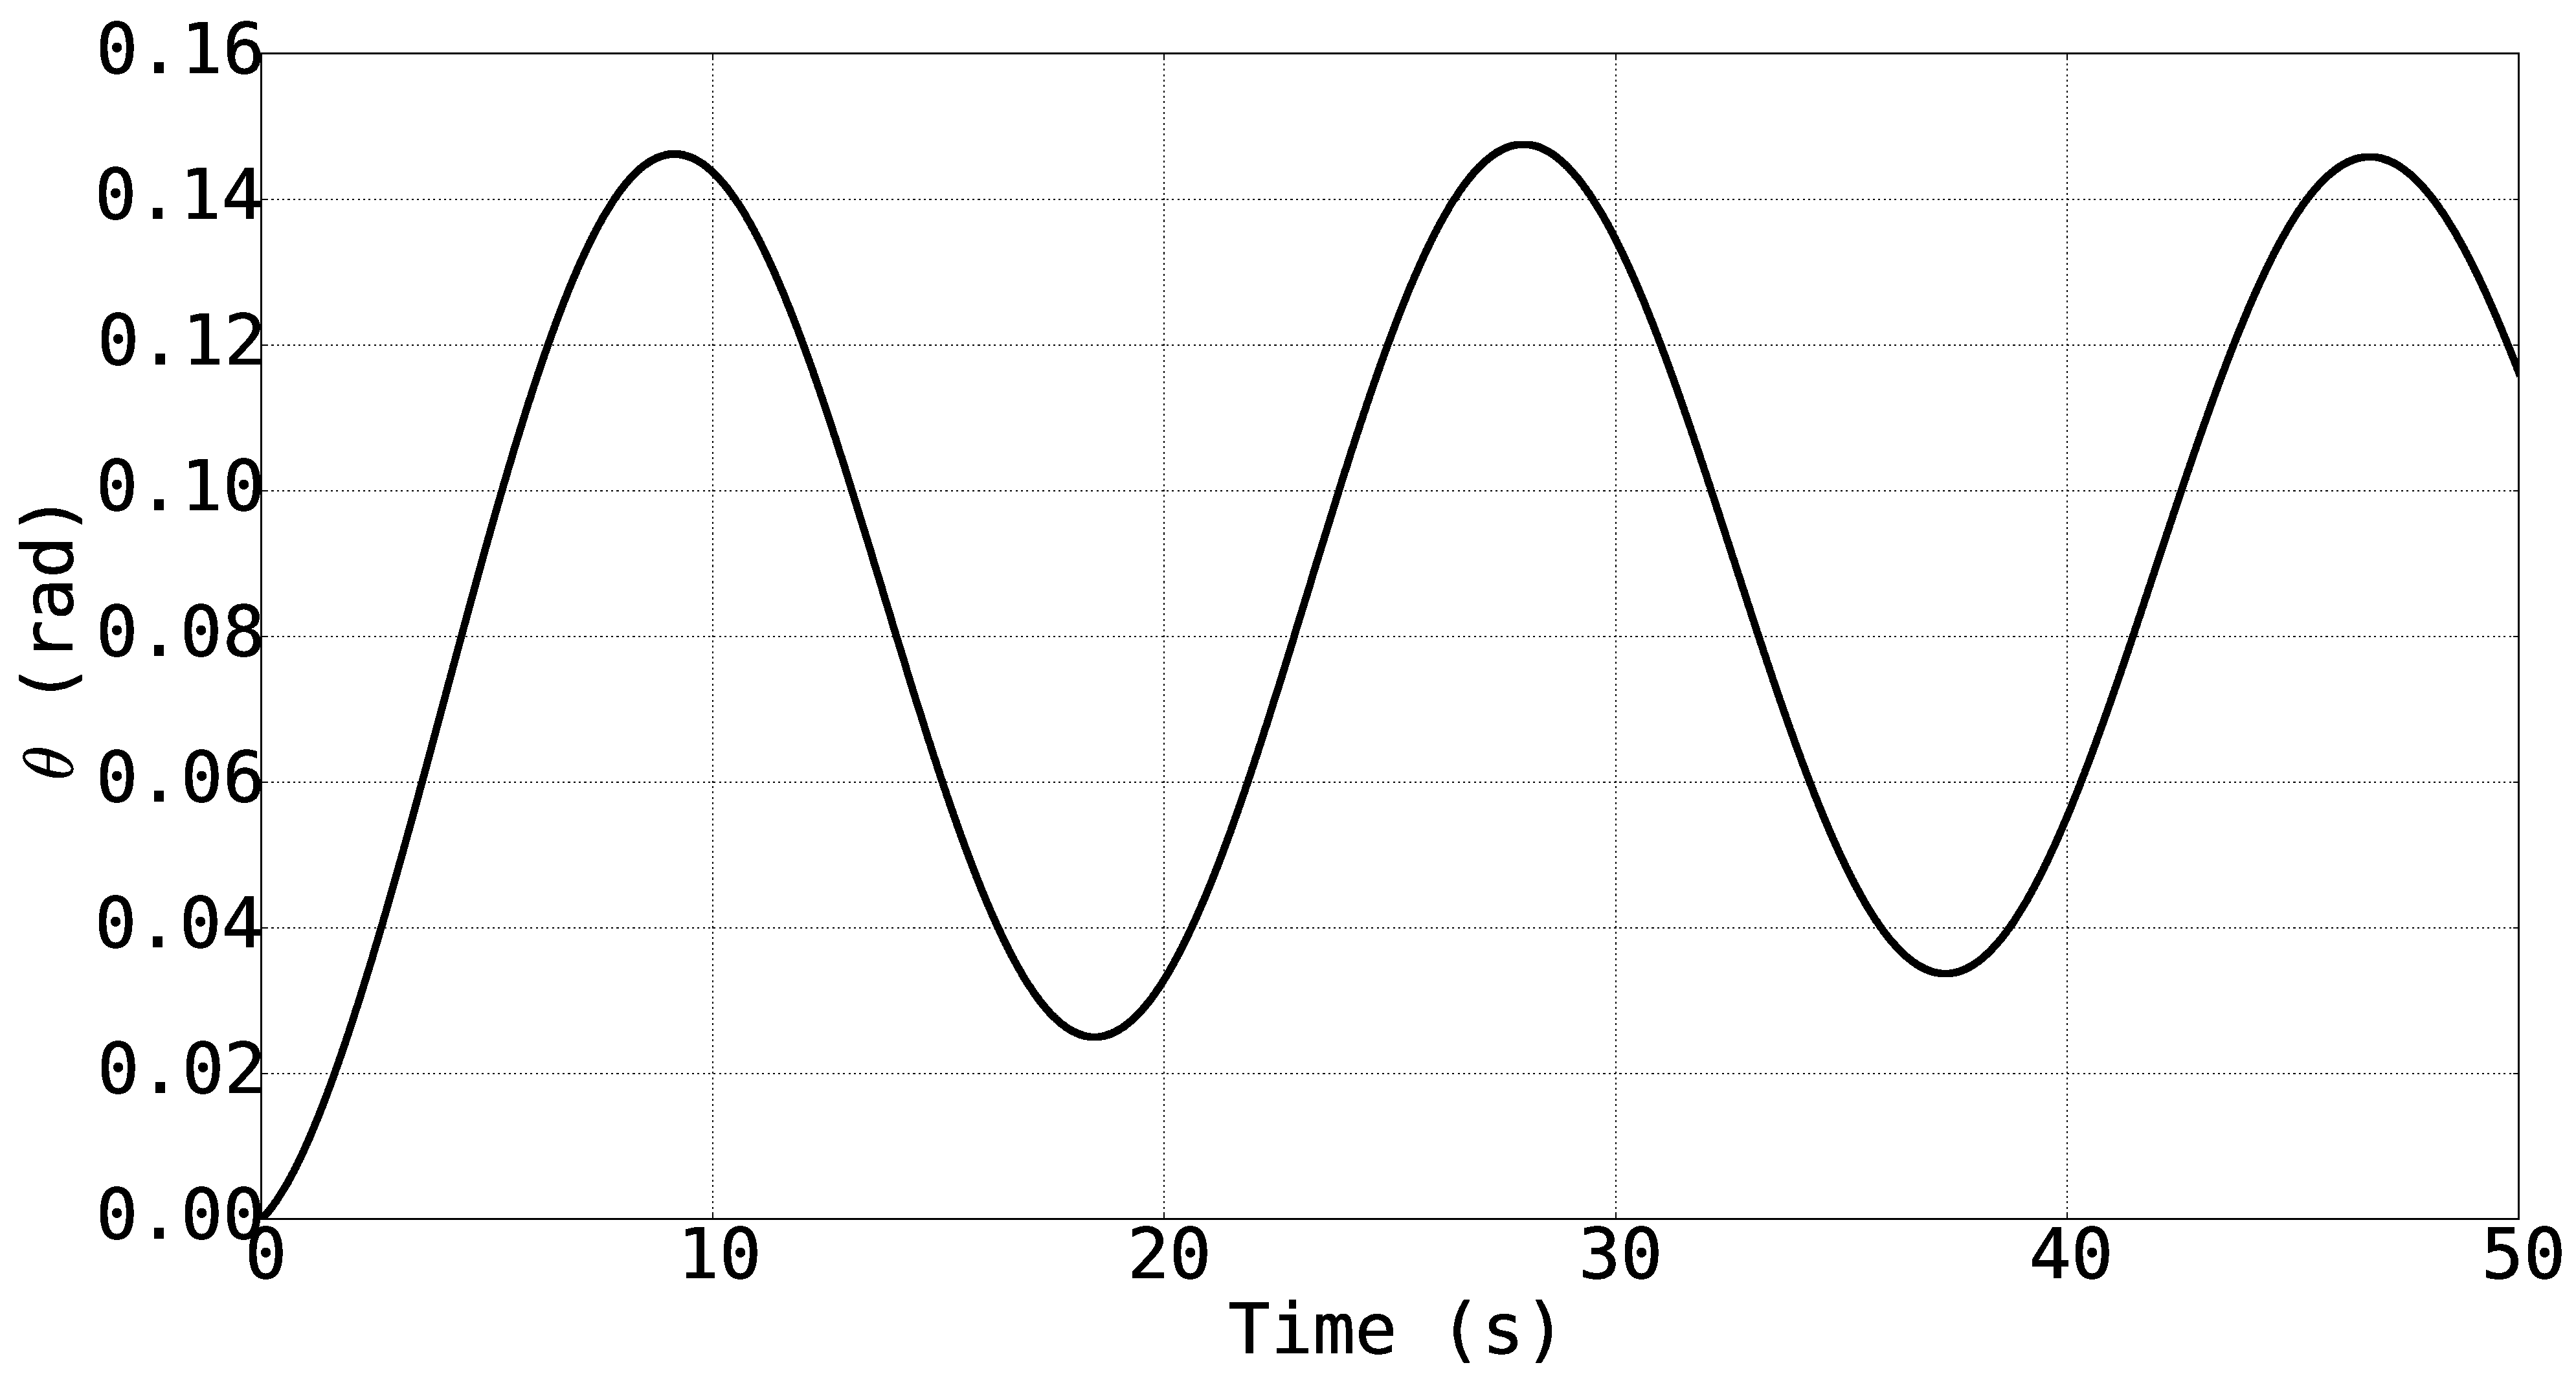
\includegraphics[width=6.5cm]{Chapter_5/figure/airfoil1_rotation.eps}
    }
    \quad
    \subfigure[Thick airfoil rotation]
    {
    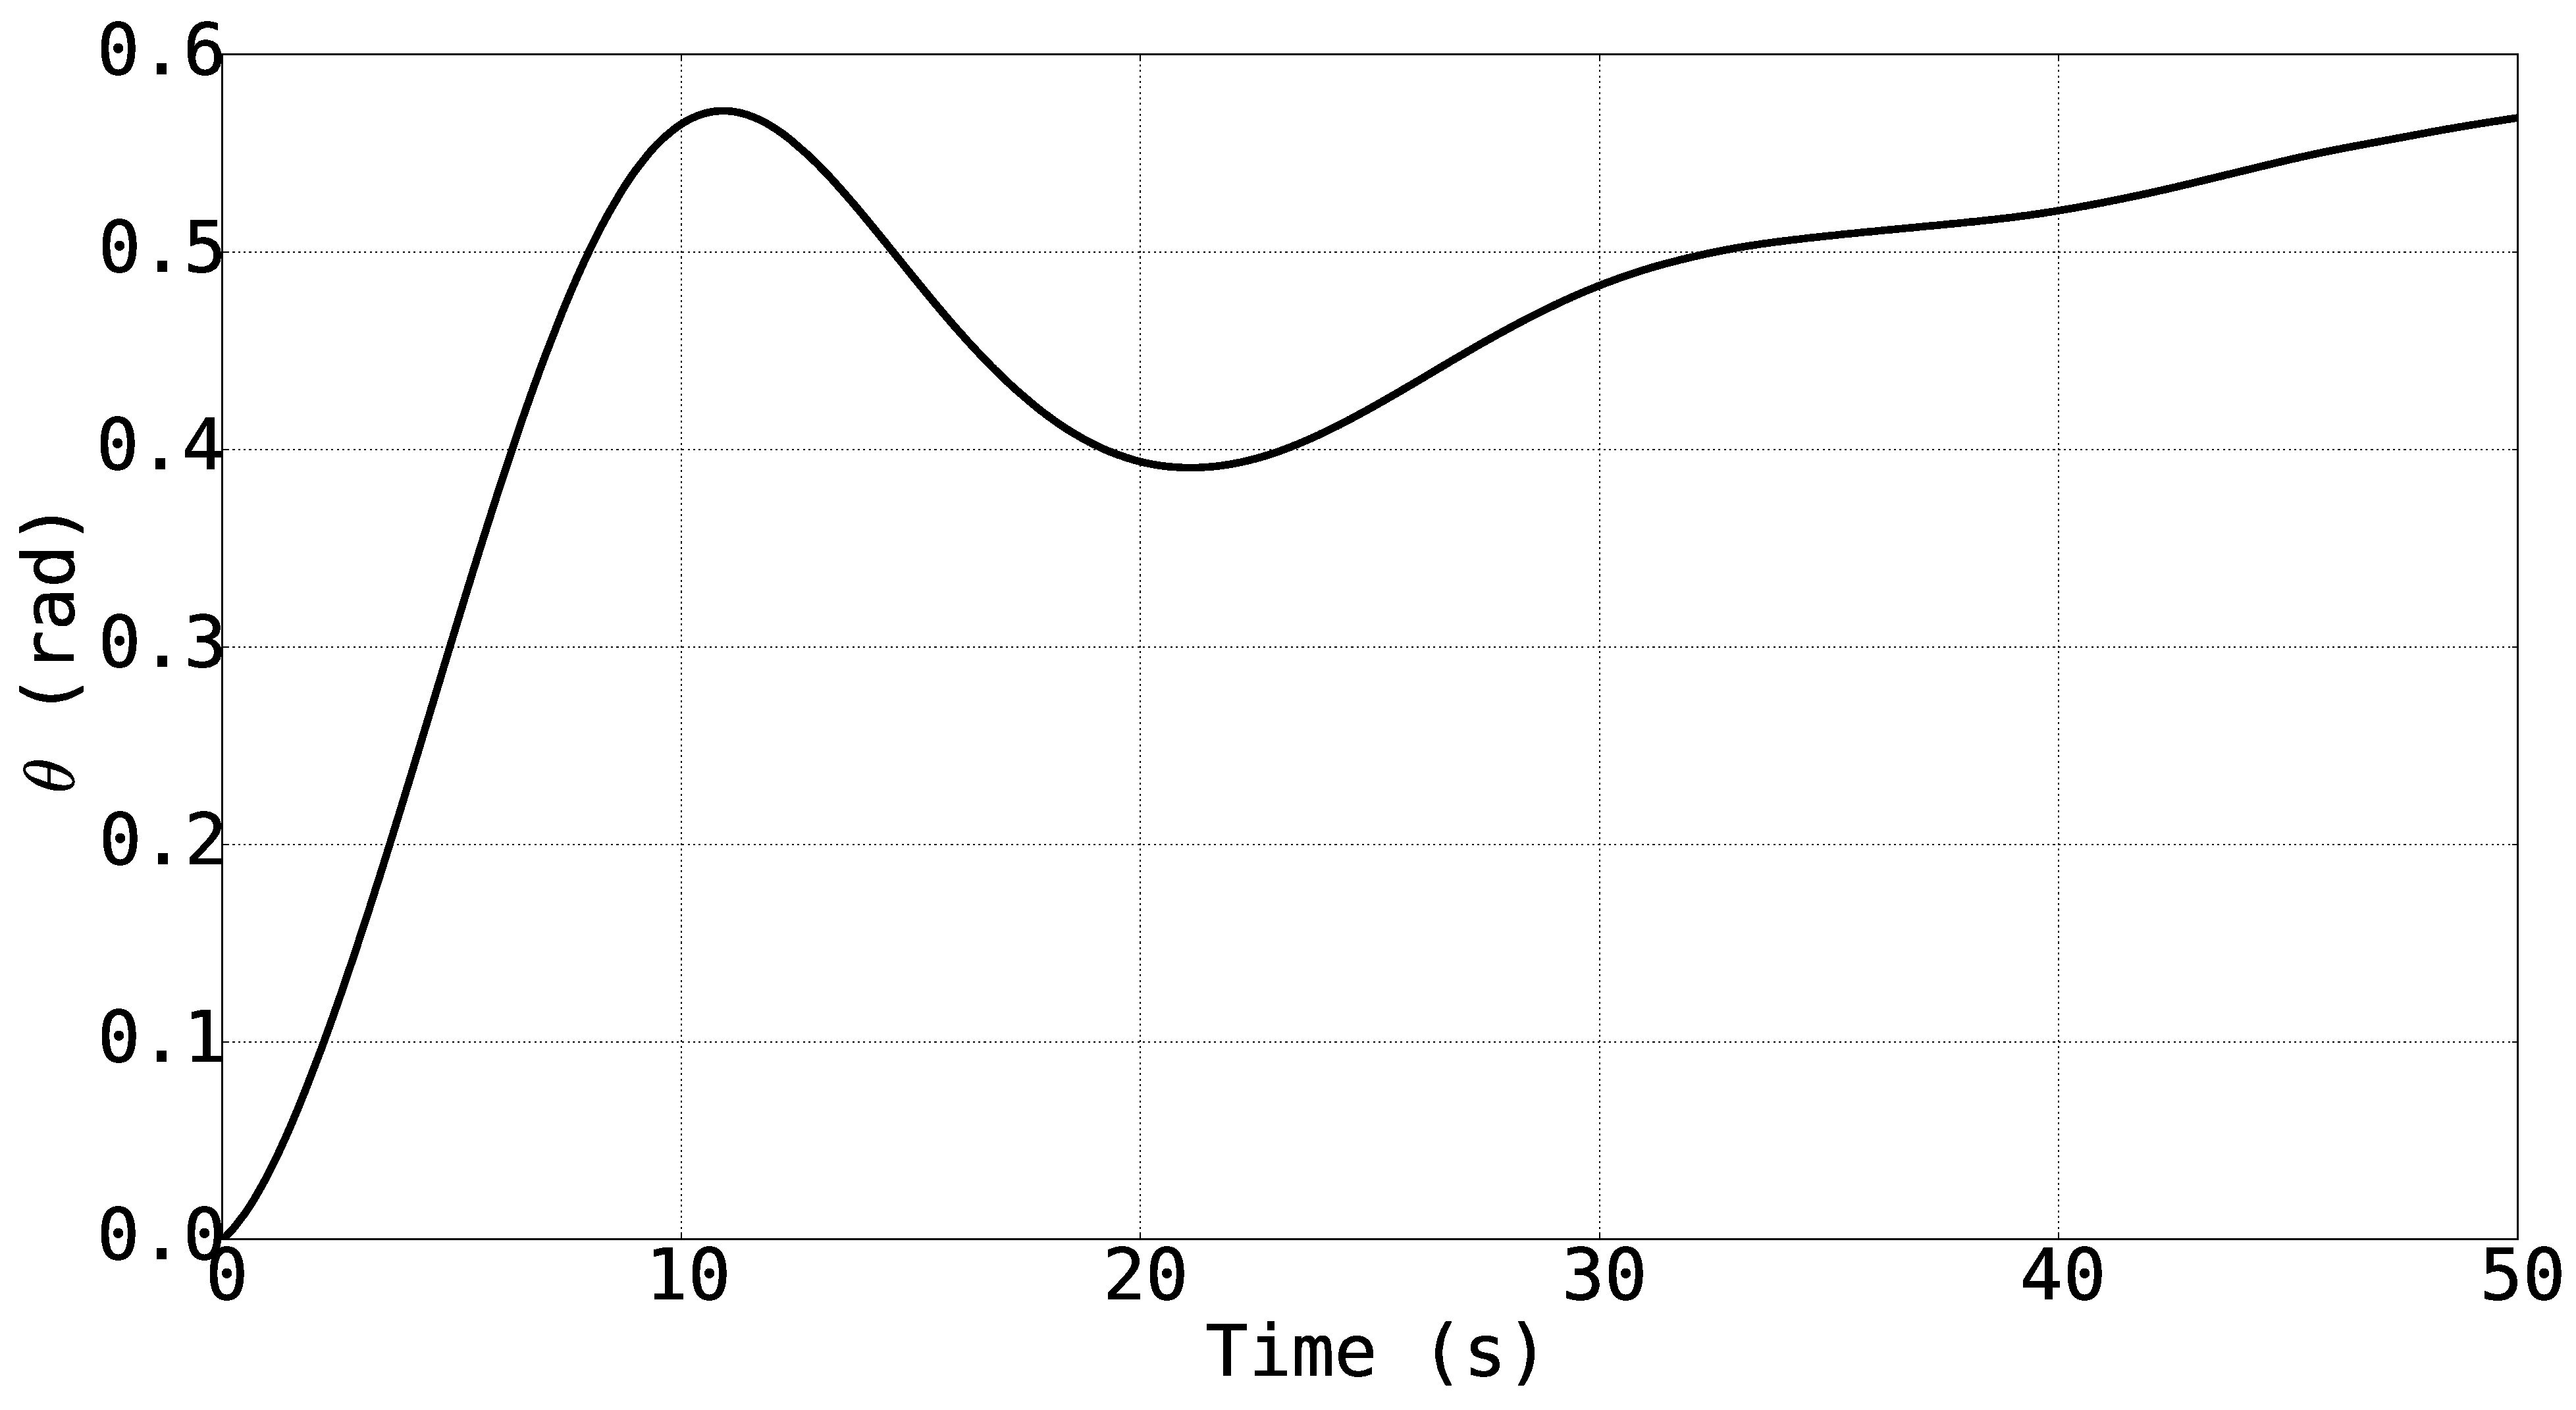
\includegraphics[width=6.5cm]{Chapter_5/figure/airfoil2_rotation.eps}
    }
    \caption{Airfoil displacement and rotation results due to aerodynamic loads.}
    \label{fig:C5_airfoilDisplacementRotation}
\end{figure}
%
To better understand the solution history, three snapshots from the u-velocity contour of the two airfoils are shown in Figure \ref{fig:C5_snapshotAirfoilSolution}. As shown here, the thick airfoil goes through large displacement and deformation. This is extremely difficult to capture using conventional body-conformal method, however can be done with rather ease by utilizing the current IB approach.
%
\begin{figure}[H]
    \centering
    \subfigure[$t = 0 \text{ sec}$]
    {
    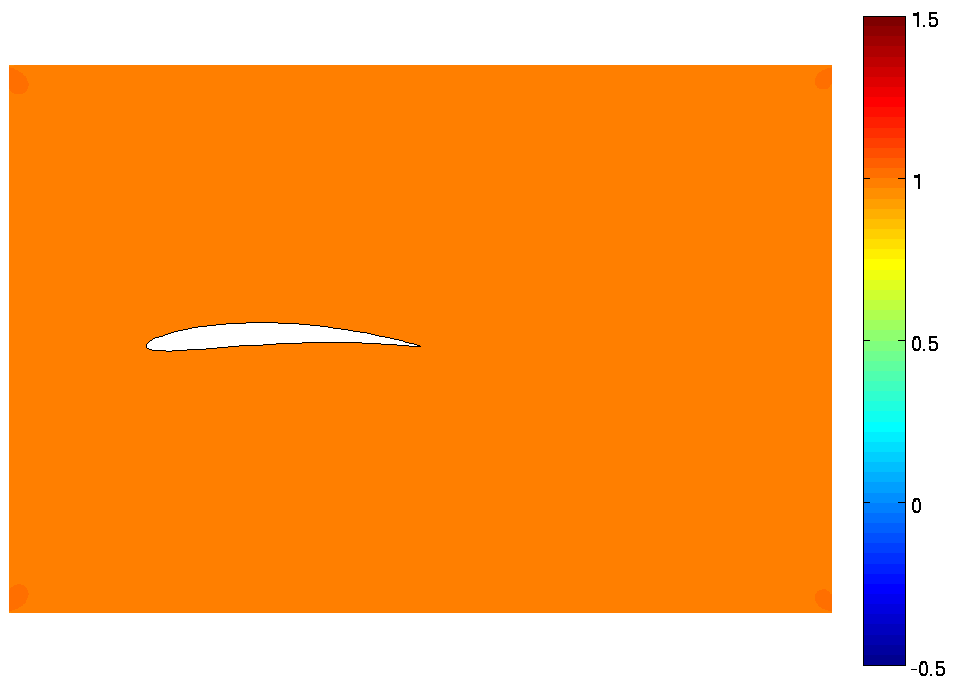
\includegraphics[width=4.25cm]{Chapter_5/figure/airfoil1_analysis_t0.png}
    }
    \quad
    \subfigure[$t = 5 \text{ sec}$]
    {
    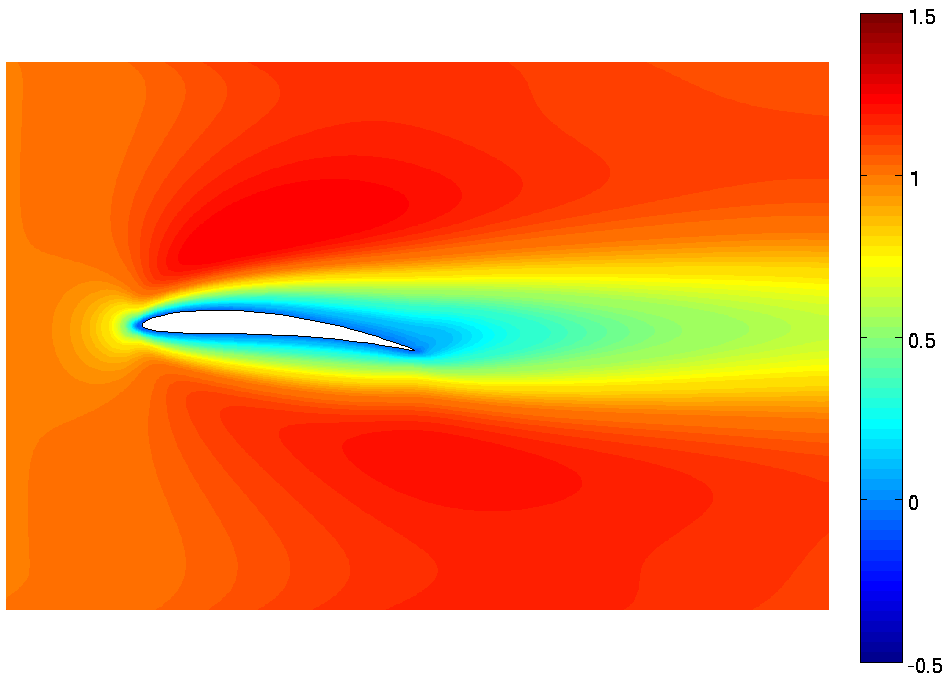
\includegraphics[width=4.25cm]{Chapter_5/figure/airfoil1_analysis_t5.png}
    }
    \quad
    \subfigure[$t = 25 \text{ sec}$]
    {
    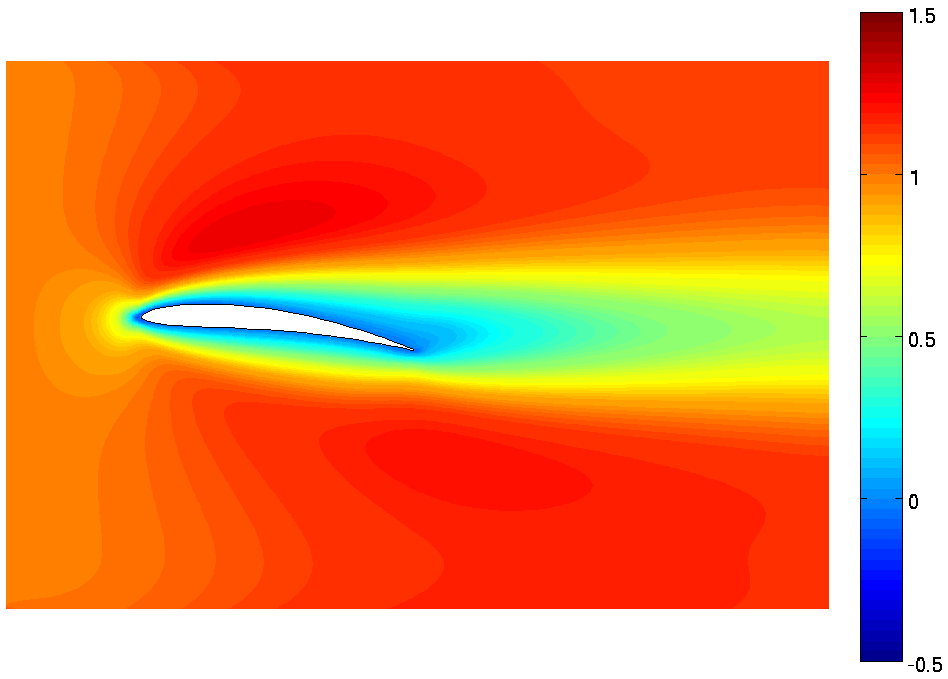
\includegraphics[width=4.25cm]{Chapter_5/figure/airfoil1_analysis_t25.png}
    }
    \\
    \subfigure[$t = 0 \text{ sec}$]
    {
    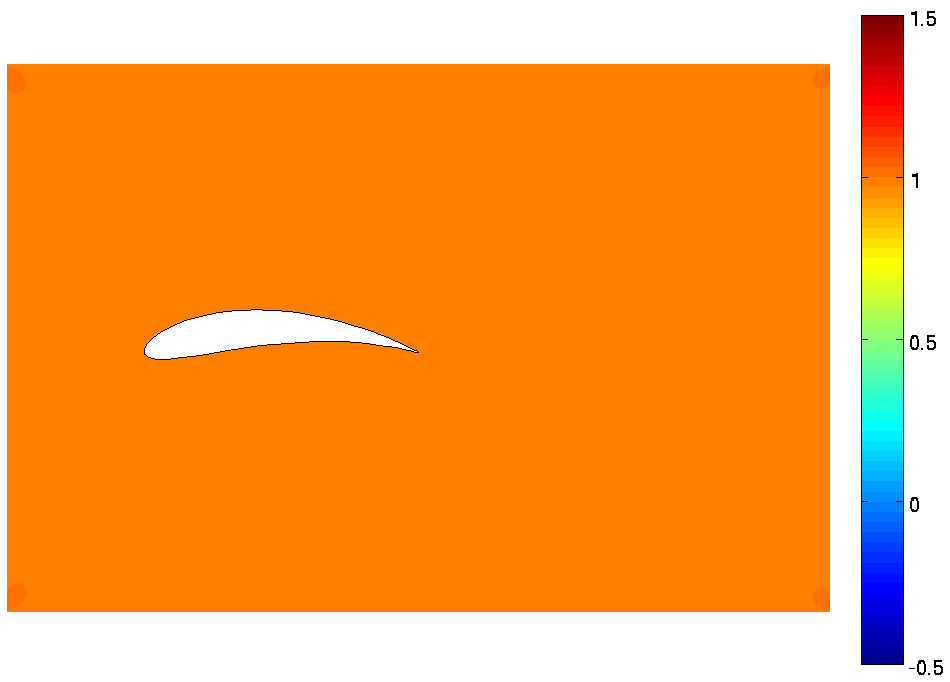
\includegraphics[width=4.25cm]{Chapter_5/figure/airfoil2_analysis_t0.png}
    }
    \quad
    \subfigure[$t = 5 \text{ sec}$]
    {
    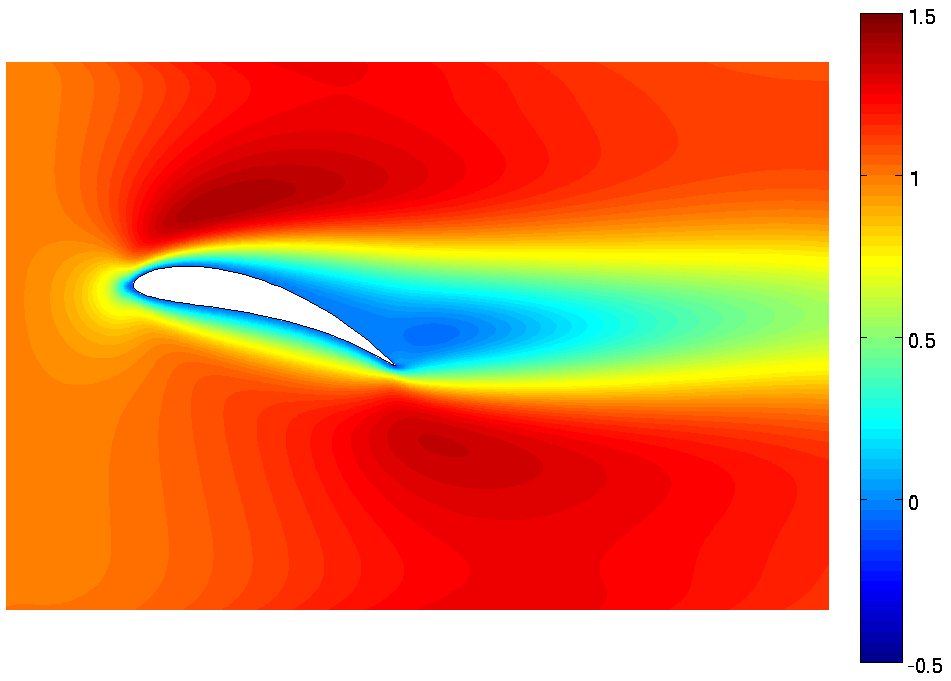
\includegraphics[width=4.25cm]{Chapter_5/figure/airfoil2_analysis_t5.png}
    }
    \quad
    \subfigure[$t = 25 \text{ sec}$]
    {
    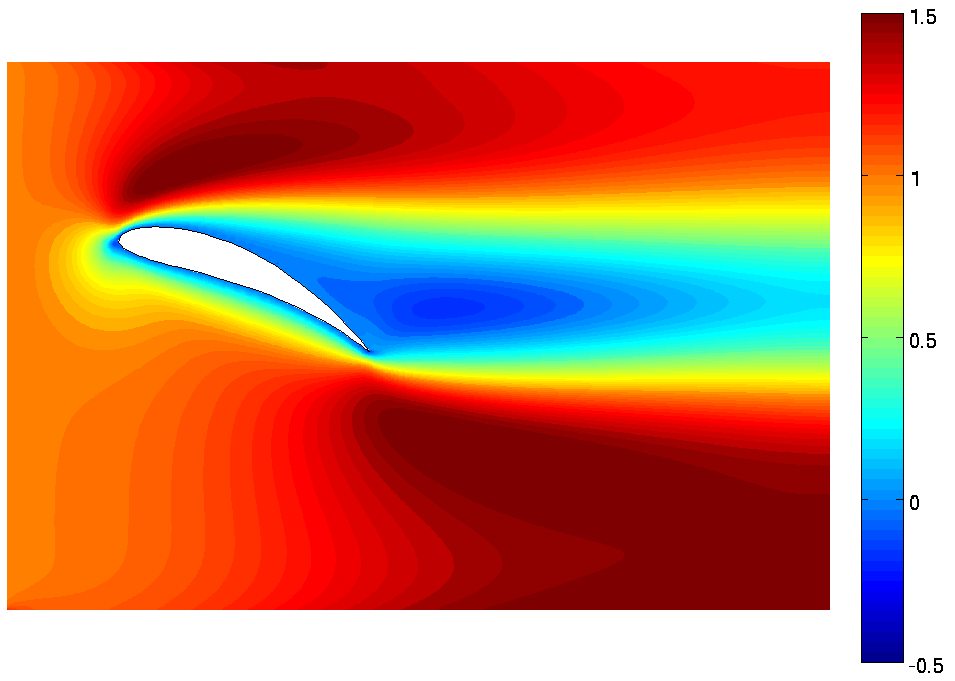
\includegraphics[width=4.25cm]{Chapter_5/figure/airfoil2_analysis_t25.png}
    }
    \caption{U-velocity time snapeshots for airfoil on elastic structure.}
    \label{fig:C5_snapshotAirfoilSolution}
\end{figure}
%
For the sensitivity analysis, we investigate the sensitivity of the airfoil displacement and rotation to change in its chamber. As discussed in Chapter \ref{ch:shapeSenwithIB}, as a part of sensitivity calculation, it is required to derive the shape sensitivities. This is done analytically since the Joukowski transform provides us with an analytical definition for the airfoil boundary. The shape sensitivity of the airfoil with respect to camber is calculated by differentiating Equation \eqref{eq:C5_joukowskyTransform} with respect to the $y$ coordinate of the center of the airfoil. For the structure side, the shape only affects the loads acting on the elastic structure and not its shape. Therefore, we can use the same solver used for calculating the displacement and rotation of the structure for the sensitivity calculation. The time history of the sensitivity results for the displacement and rotation of the two airfoils is shown in Figure \ref{fig:C5_airfoilSensitivityTimeHistory}.
%
\begin{figure}[H]
    \centering
    \subfigure[Thin airfoil displacement sensitivity]
    {
    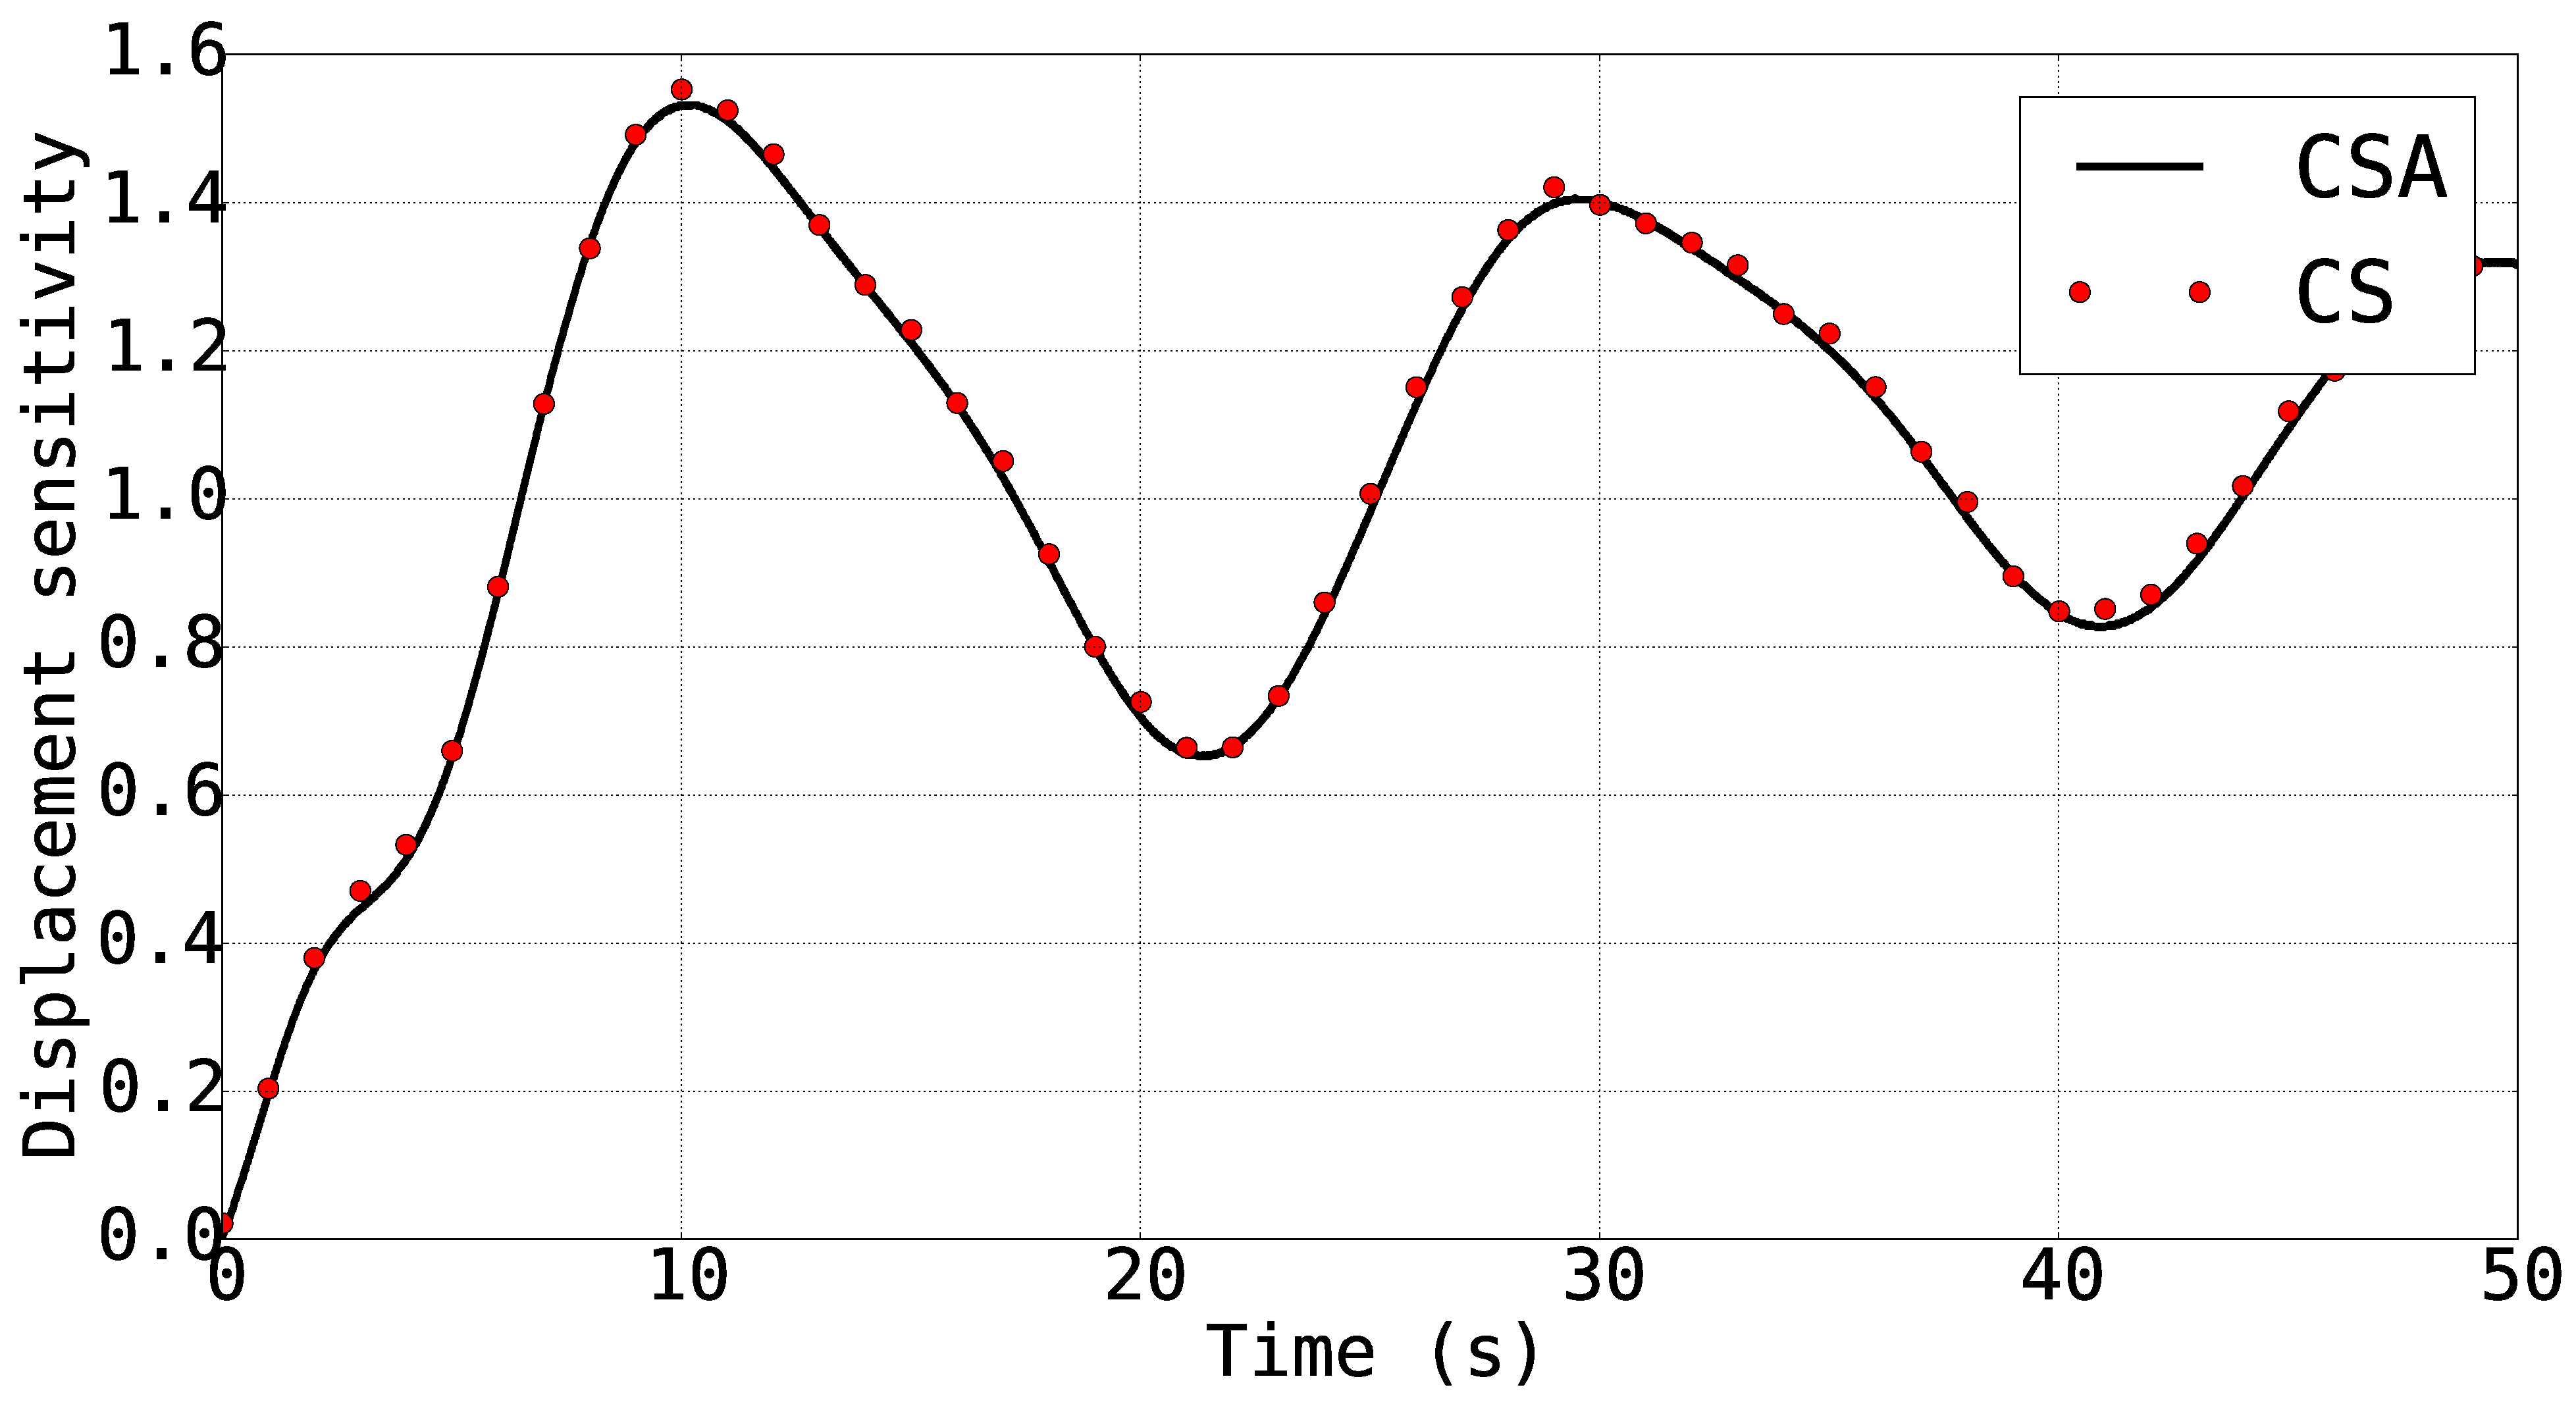
\includegraphics[width=6.5cm]{Chapter_5/figure/airfoil1_disp_sensitivity.eps}
    }
    \quad
    \subfigure[Thick airfoil displacement sensitivity]
    {
    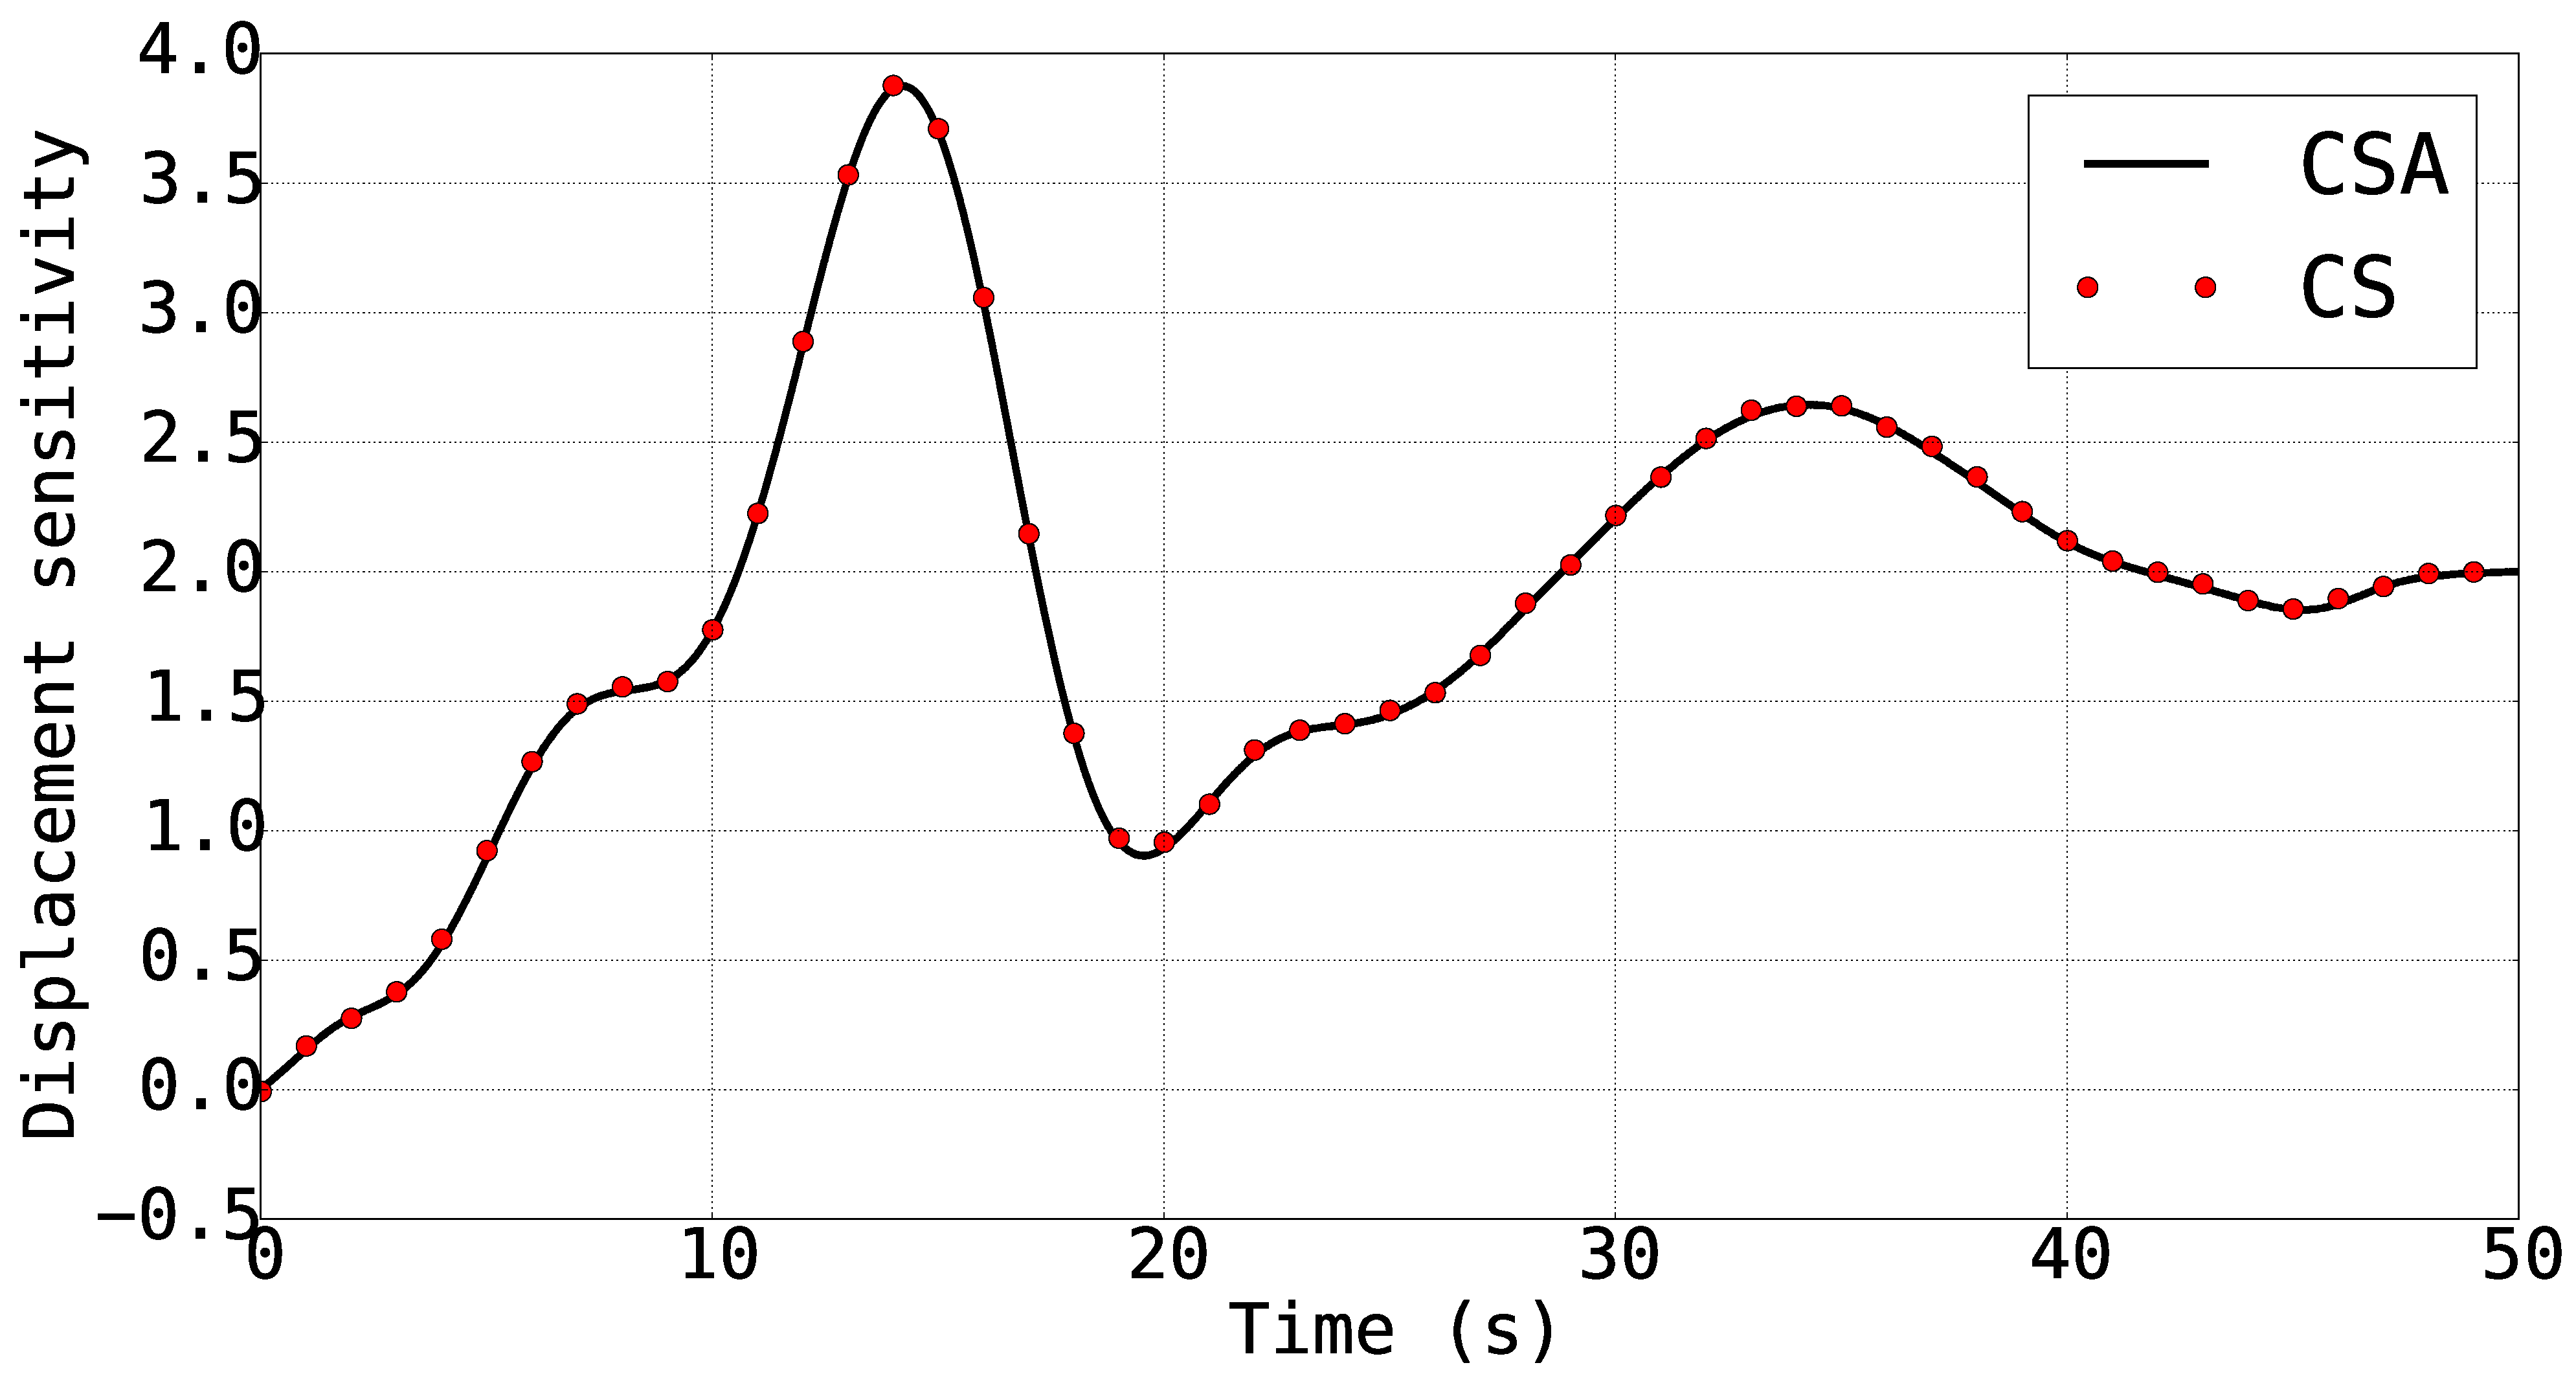
\includegraphics[width=6.5cm]{Chapter_5/figure/airfoil2_disp_sensitivity.eps}
    }
    \\
    \subfigure[Thin airfoil rotation sensitivity]
    {
    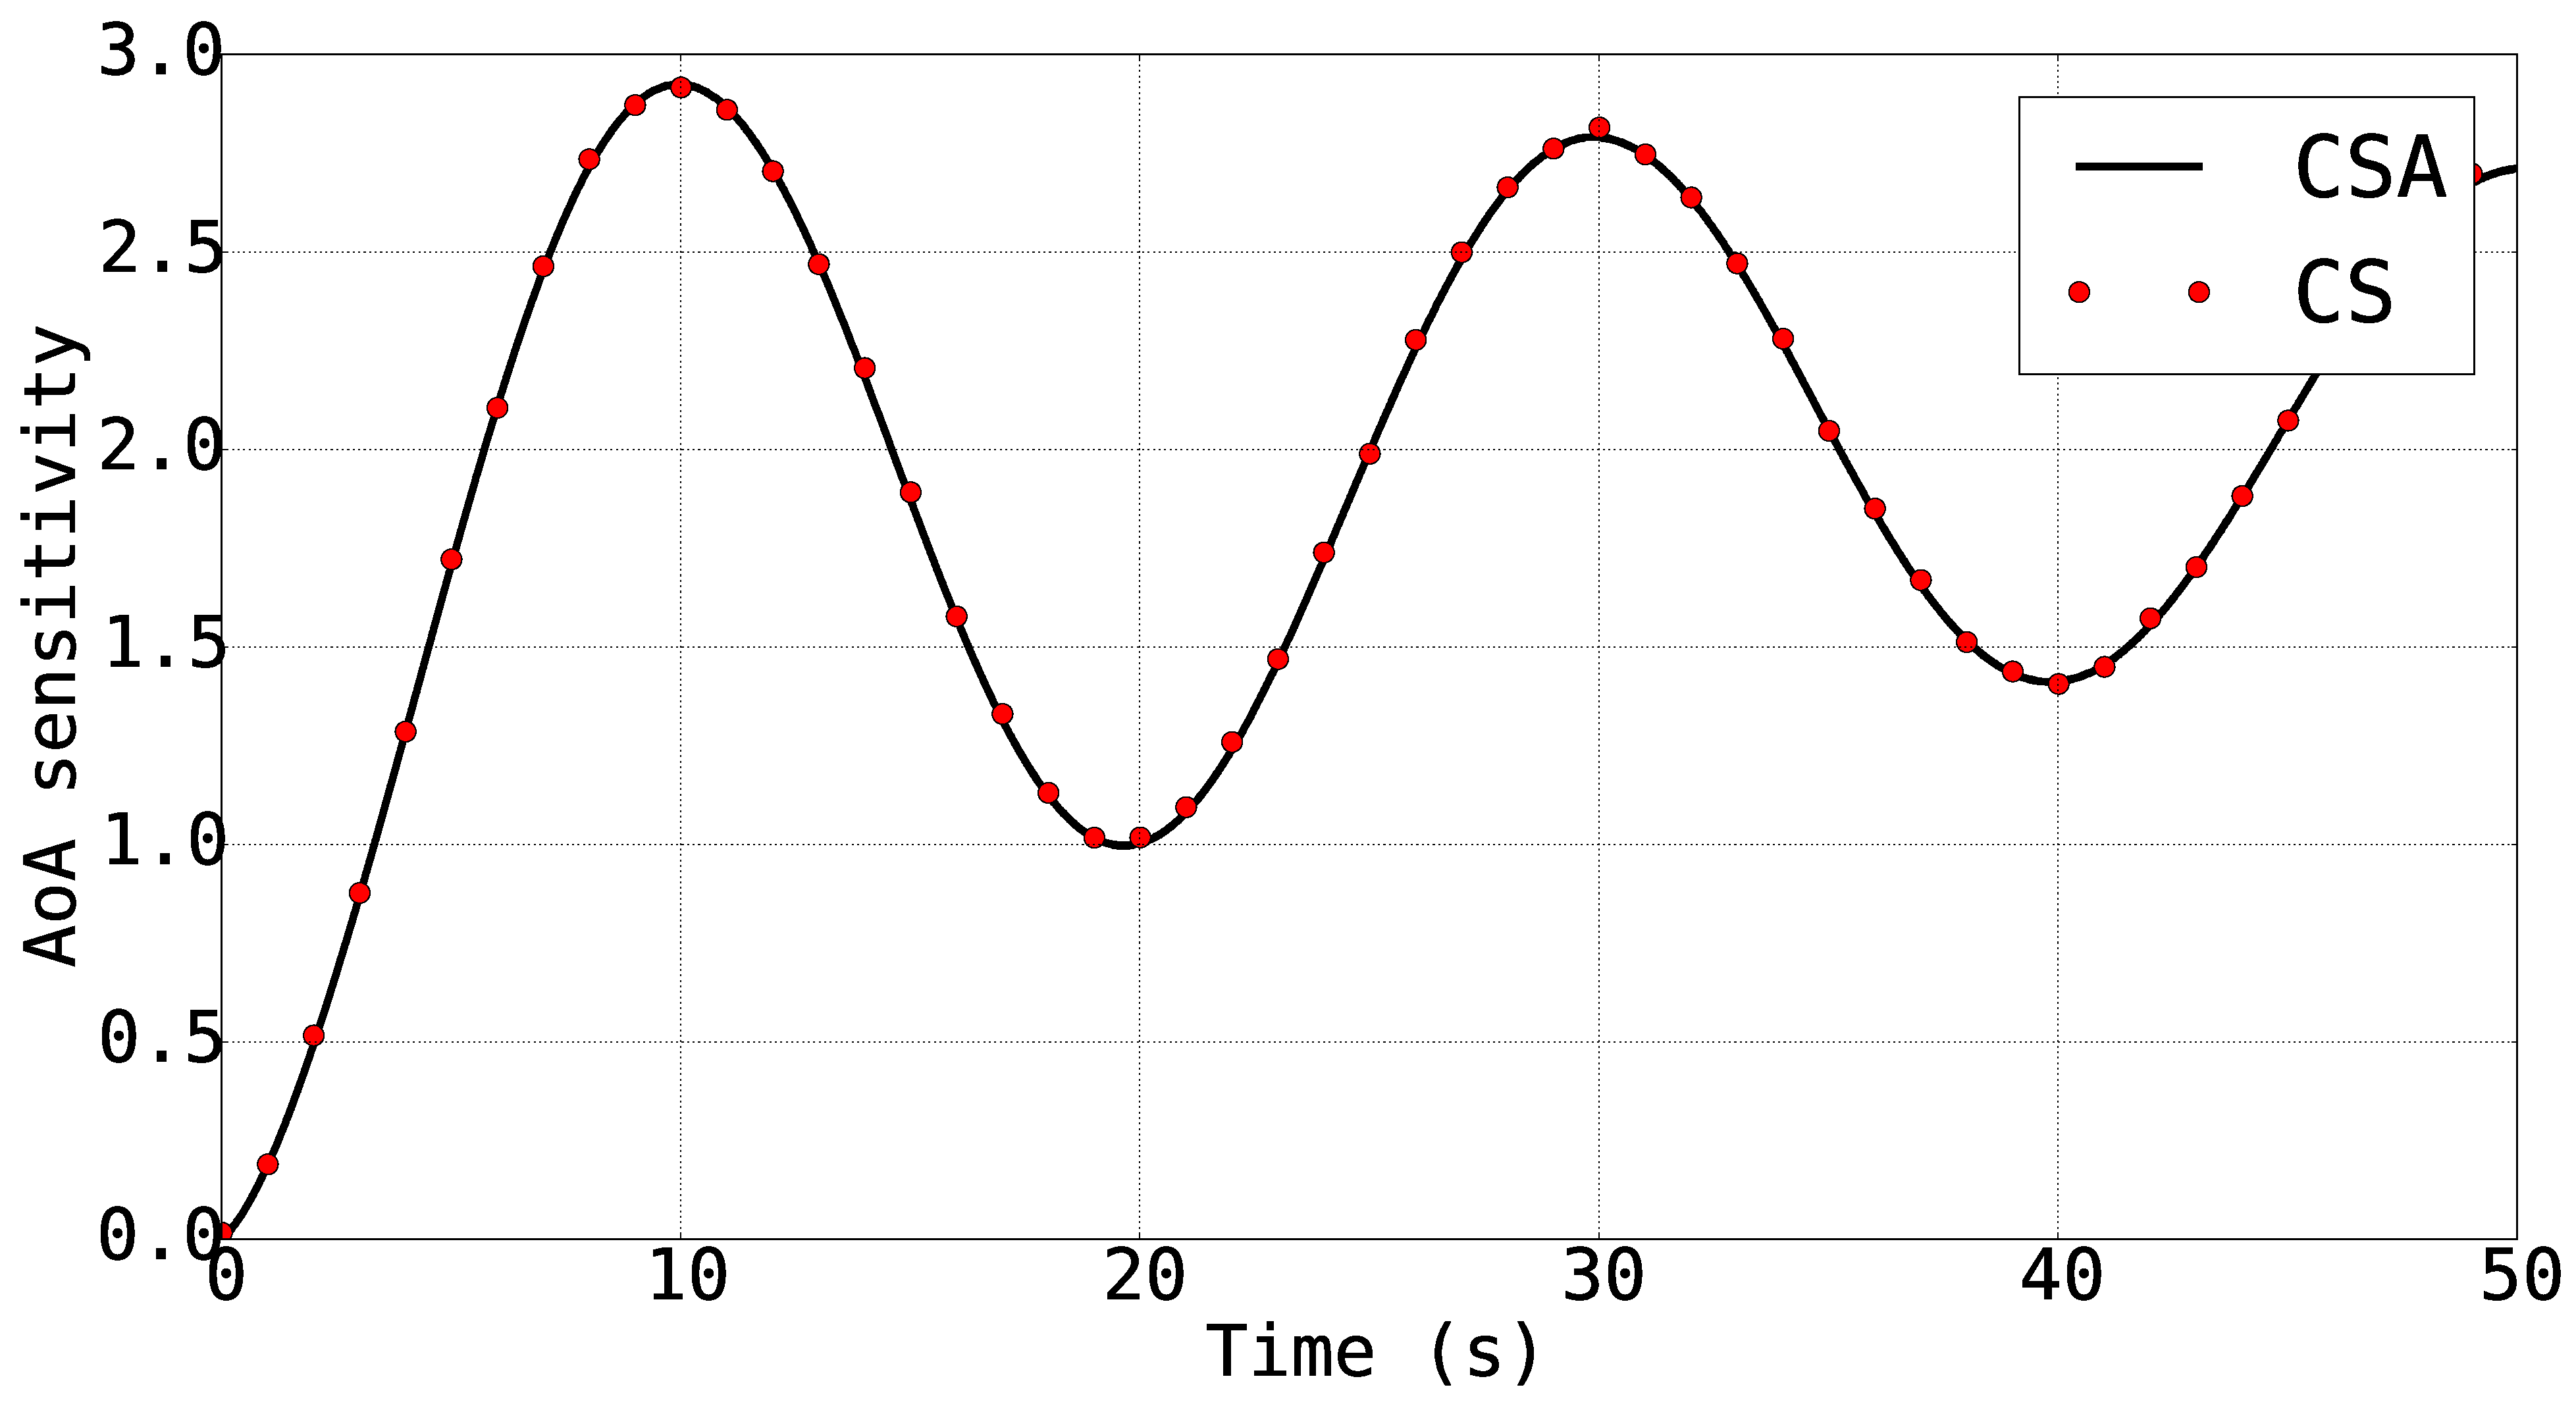
\includegraphics[width=6.5cm]{Chapter_5/figure/airfoil1_rotation_sensitivity.eps}
    }
    \quad
    \subfigure[Thick airfoil rotation sensitivity]
    {
    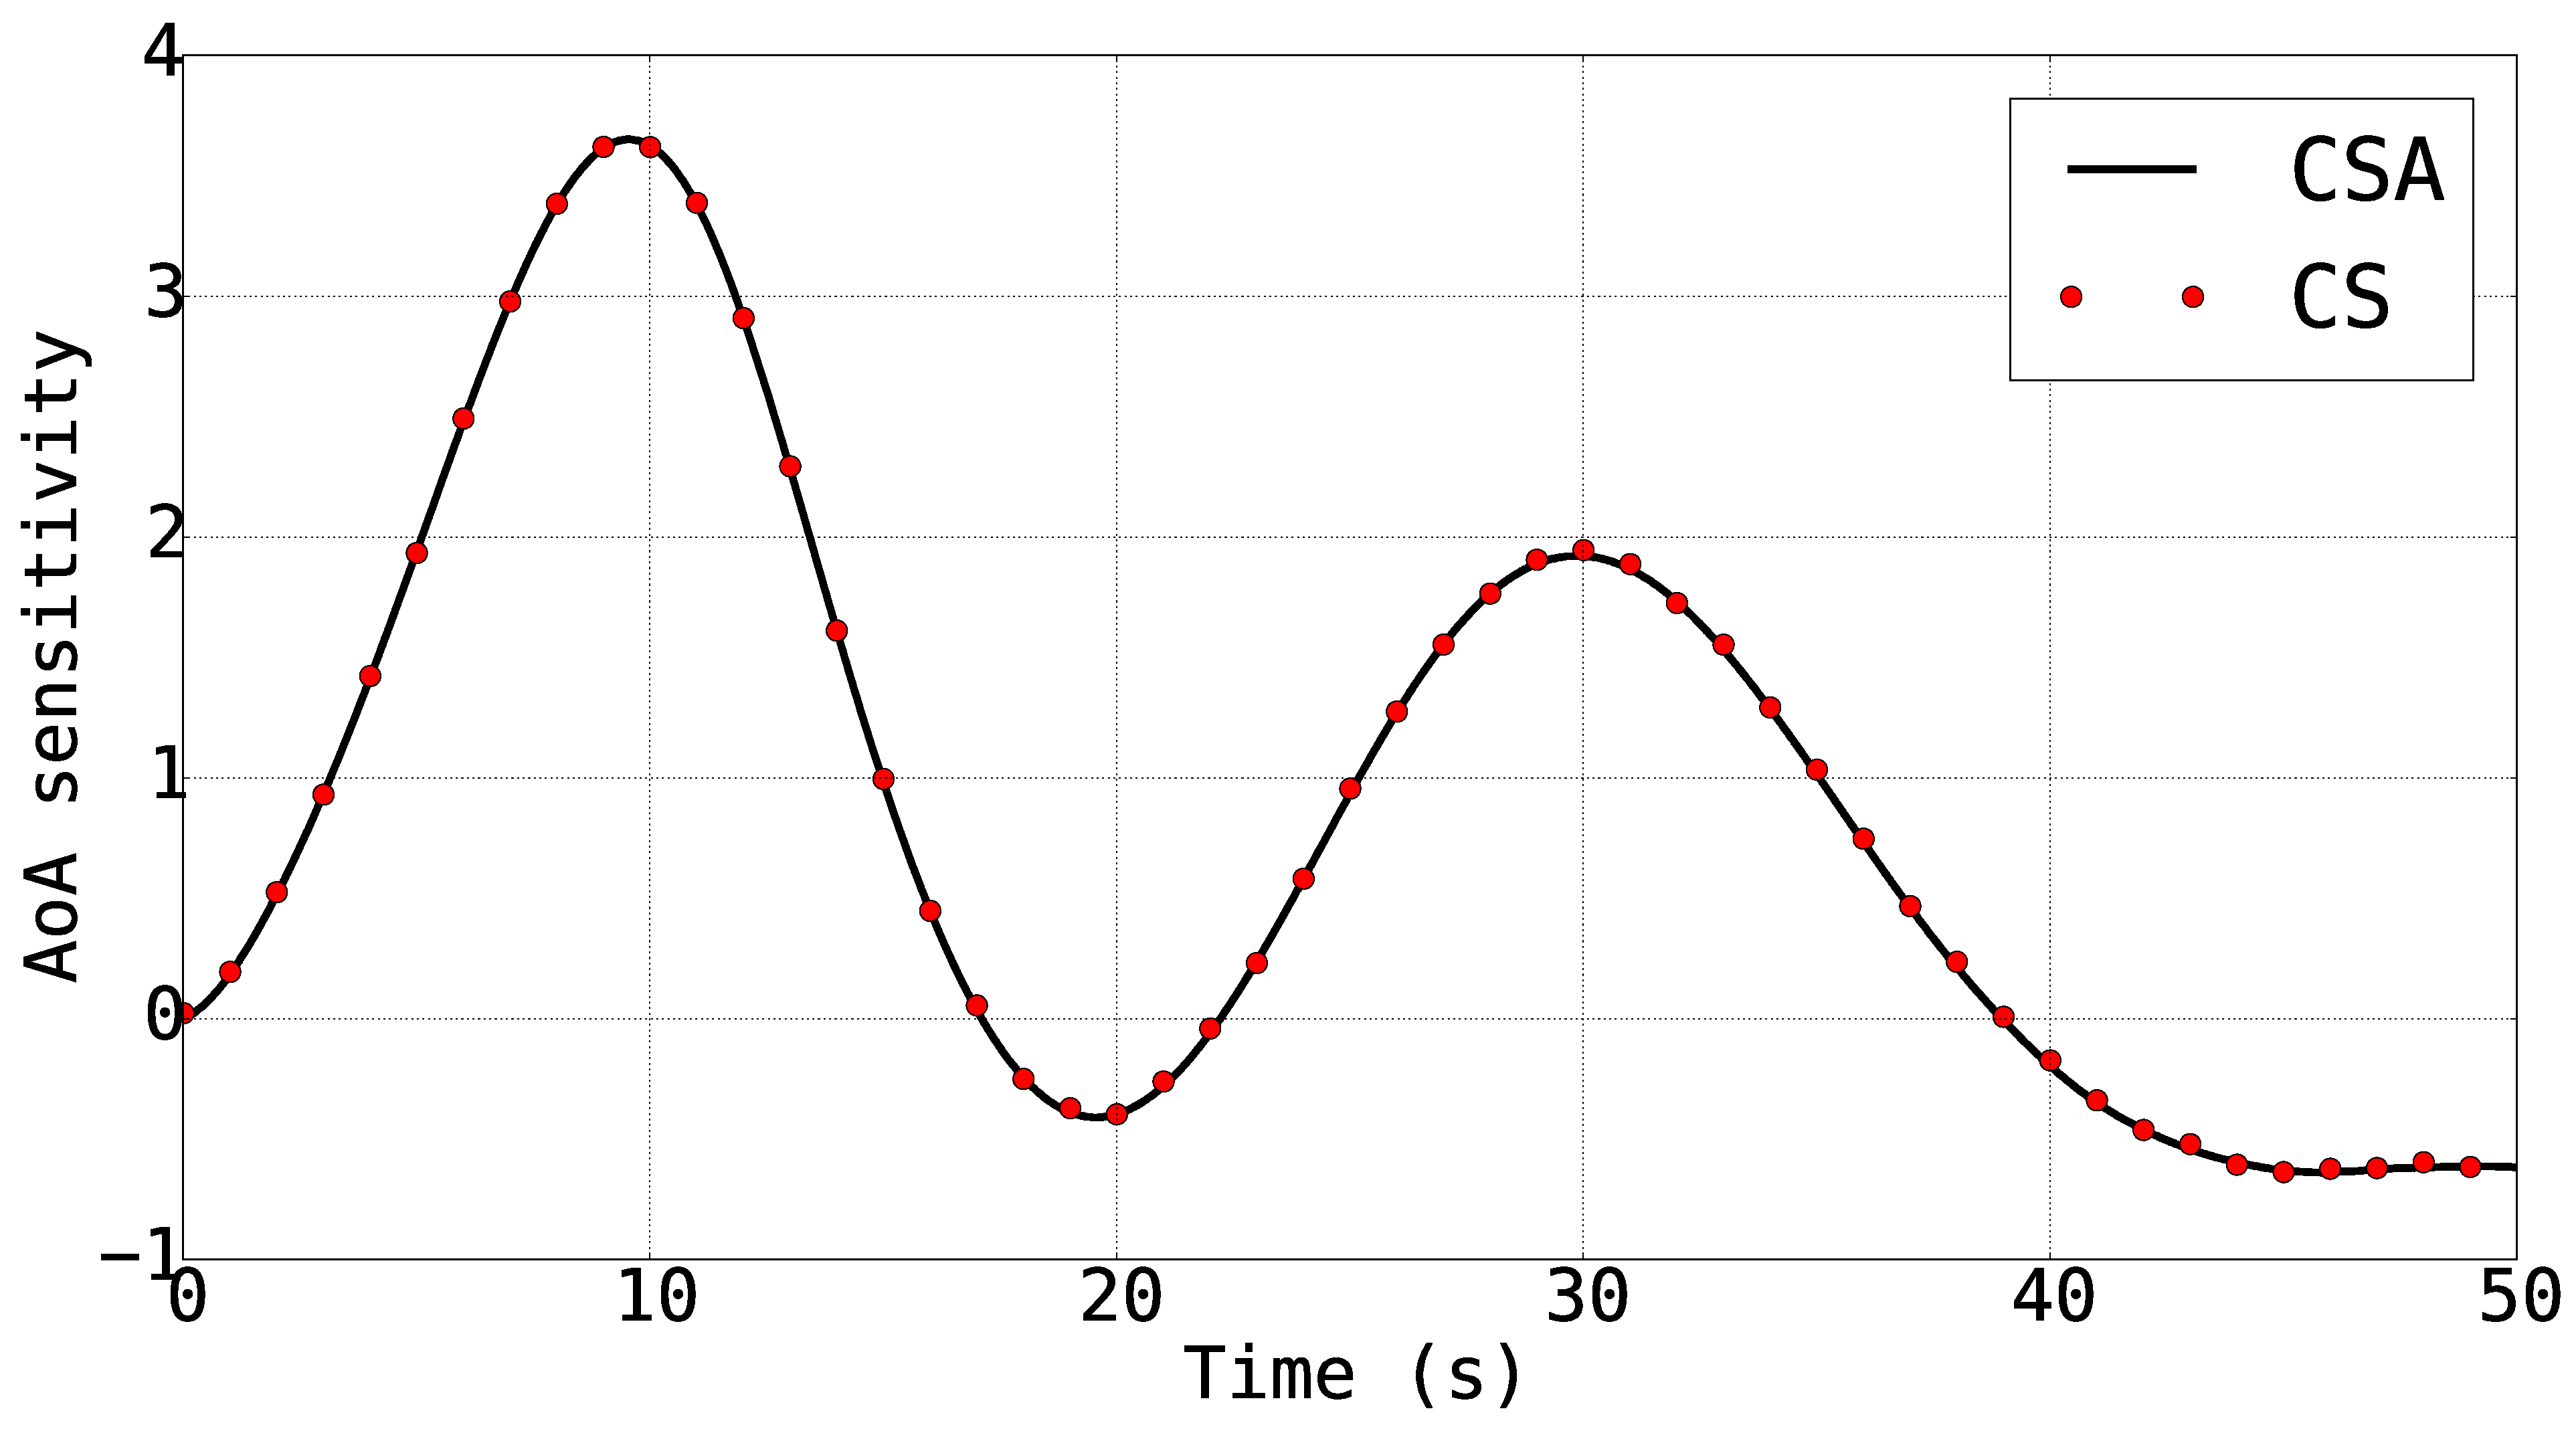
\includegraphics[width=6.5cm]{Chapter_5/figure/airfoil2_rotation_sensitivity.eps}
    }
    \caption{Airfoil displacement and rotation sensitivity results due to change in camber.}
    \label{fig:C5_airfoilSensitivityTimeHistory}
\end{figure}
%
As shown in Figure \ref{fig:C5_airfoilSensitivityTimeHistory}, the sensitivity response flows the same pattern as the analysis solution for this problem. For the oscillatory response of the thin airfoil, the sensitivity solution also moves between two extremes for both the displacement and airfoil rotation. However, for the thick airfoil that shows a divergence charachteristic as shown in Figure \ref{fig:C5_airfoilDisplacementRotation}, the sensitivities also reach a constant value. It is interesting to see that for the thick airfoil, by increasing the thickness the lift will increase and therefore we see positive sensitivities for the displacement; however, the moment generated around the quarter chord decreases which causes a negative sensitivity for the rotation.

Finally, we looked at the u-velocity sensitivity contours as shown in Figure \ref{fig:C5_airfoilSensitivityContour} for different snapshots in time. As shown here, the velocity field around the airfoil in both cases as the most sensitivity near the tip.
%
\begin{figure}[H]
    \centering
    \subfigure[$t = 0 \text{ sec}$]
    {
    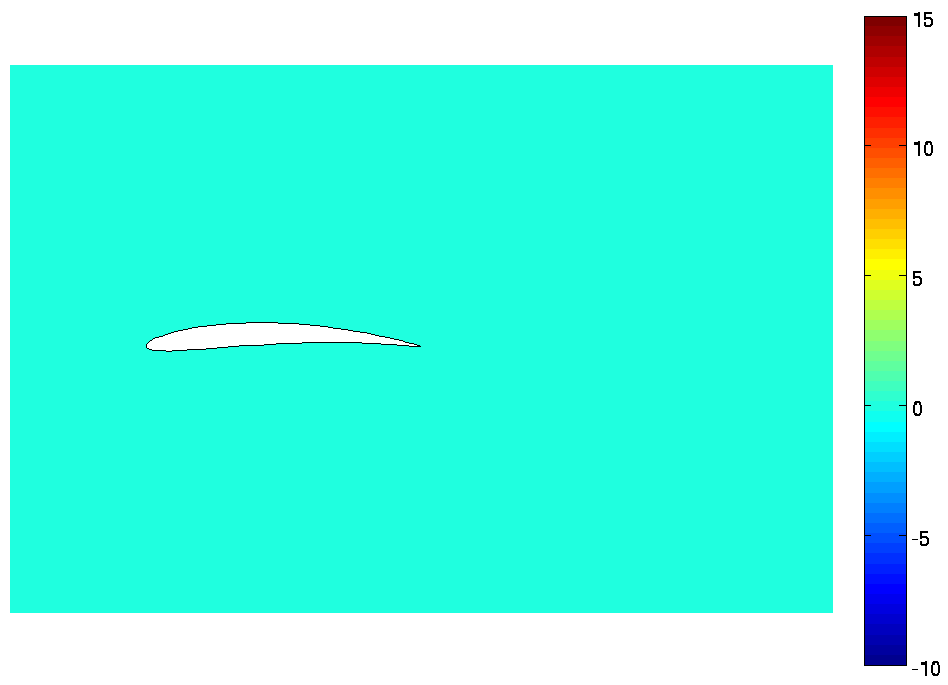
\includegraphics[width=4.25cm]{Chapter_5/figure/airfoil1_sensitivity_t0.png}
    }
    \quad
    \subfigure[$t = 5 \text{ sec}$]
    {
    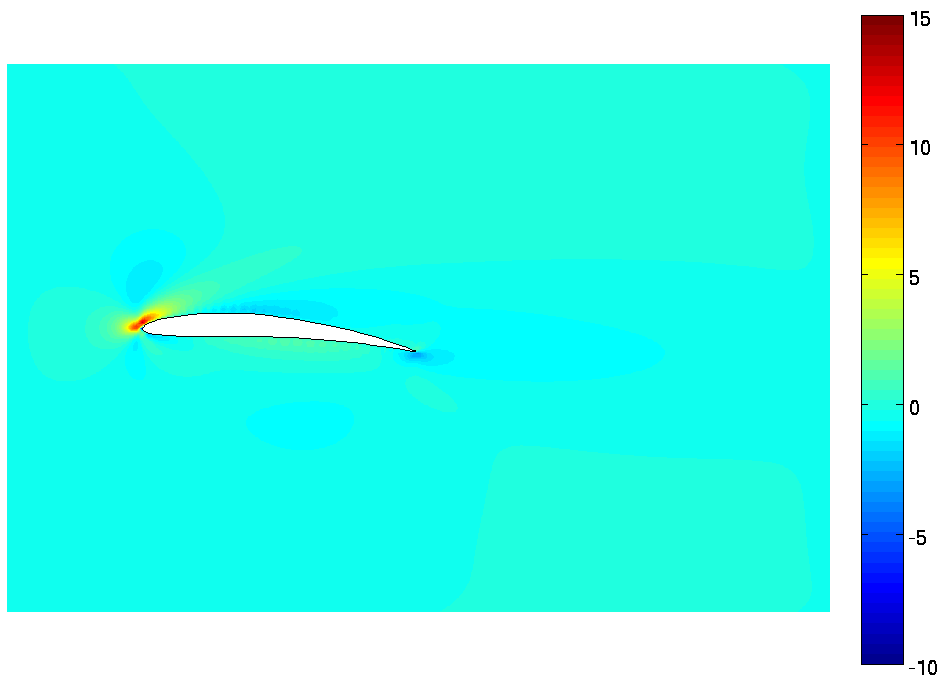
\includegraphics[width=4.25cm]{Chapter_5/figure/airfoil1_sensitivity_t5.png}
    }
    \quad
    \subfigure[$t = 25 \text{ sec}$]
    {
    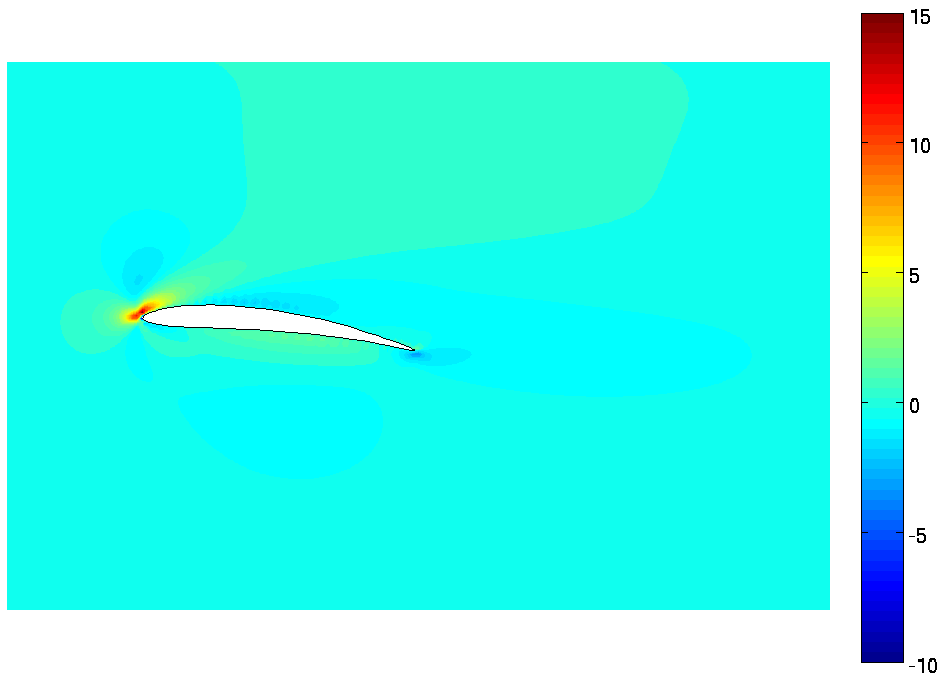
\includegraphics[width=4.25cm]{Chapter_5/figure/airfoil1_sensitivity_t25.png}
    }
    \\
    \subfigure[$t = 0 \text{ sec}$]
    {
    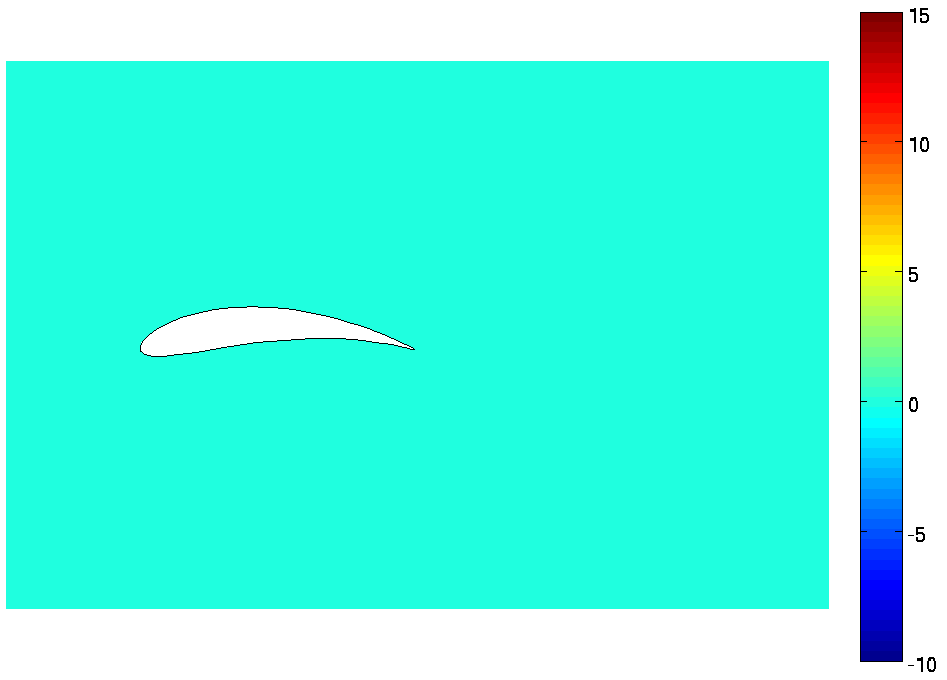
\includegraphics[width=4.25cm]{Chapter_5/figure/airfoil2_sensitivity_t0.png}
    }
    \quad
    \subfigure[$t = 5 \text{ sec}$]
    {
    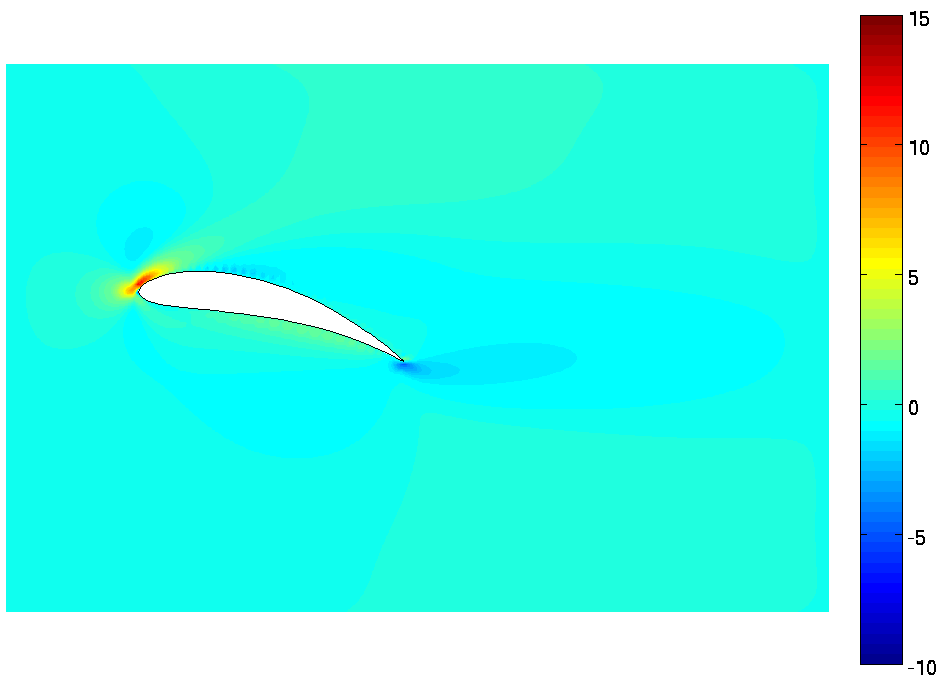
\includegraphics[width=4.25cm]{Chapter_5/figure/airfoil2_sensitivity_t5.png}
    }
    \quad
    \subfigure[$t = 25 \text{ sec}$]
    {
    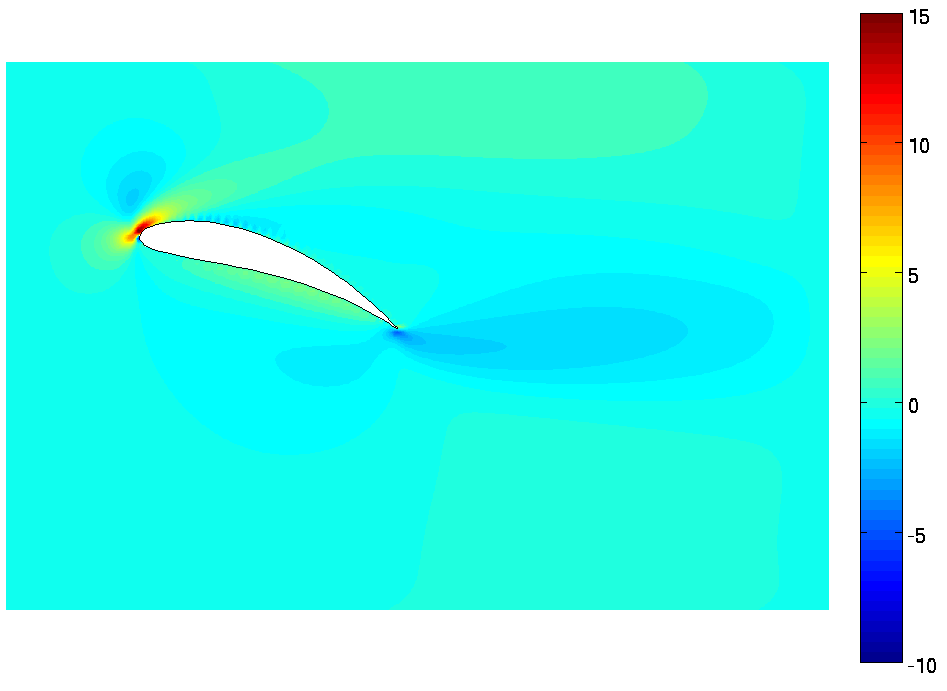
\includegraphics[width=4.25cm]{Chapter_5/figure/airfoil2_sensitivity_t25.png}
    }
    \caption{U-velocity sensitivity time snapeshots for airfoil on elastic structure.}
    \label{fig:C5_airfoilSensitivityContour}
\end{figure}
%